\documentclass[twoside]{book}

% Packages required by doxygen
\usepackage{calc}
\usepackage{doxygen}
\usepackage{graphicx}
\usepackage[utf8]{inputenc}
\usepackage{makeidx}
\usepackage{multicol}
\usepackage{multirow}
\usepackage{textcomp}
\usepackage[table]{xcolor}

% Font selection
\usepackage[T1]{fontenc}
\usepackage{mathptmx}
\usepackage[scaled=.90]{helvet}
\usepackage{courier}
\usepackage{amssymb}
\usepackage{sectsty}
\renewcommand{\familydefault}{\sfdefault}
\allsectionsfont{%
  \fontseries{bc}\selectfont%
  \color{darkgray}%
}
\renewcommand{\DoxyLabelFont}{%
  \fontseries{bc}\selectfont%
  \color{darkgray}%
}

% Page & text layout
\usepackage{geometry}
\geometry{%
  a4paper,%
  top=2.5cm,%
  bottom=2.5cm,%
  left=2.5cm,%
  right=2.5cm%
}
\tolerance=750
\hfuzz=15pt
\hbadness=750
\setlength{\emergencystretch}{15pt}
\setlength{\parindent}{0cm}
\setlength{\parskip}{0.2cm}
\makeatletter
\renewcommand{\paragraph}{%
  \@startsection{paragraph}{4}{0ex}{-1.0ex}{1.0ex}{%
    \normalfont\normalsize\bfseries\SS@parafont%
  }%
}
\renewcommand{\subparagraph}{%
  \@startsection{subparagraph}{5}{0ex}{-1.0ex}{1.0ex}{%
    \normalfont\normalsize\bfseries\SS@subparafont%
  }%
}
\makeatother

% Headers & footers
\usepackage{fancyhdr}
\pagestyle{fancyplain}
\fancyhead[LE]{\fancyplain{}{\bfseries\thepage}}
\fancyhead[CE]{\fancyplain{}{}}
\fancyhead[RE]{\fancyplain{}{\bfseries\leftmark}}
\fancyhead[LO]{\fancyplain{}{\bfseries\rightmark}}
\fancyhead[CO]{\fancyplain{}{}}
\fancyhead[RO]{\fancyplain{}{\bfseries\thepage}}
\fancyfoot[LE]{\fancyplain{}{}}
\fancyfoot[CE]{\fancyplain{}{}}
\fancyfoot[RE]{\fancyplain{}{\bfseries\scriptsize Generated on Wed Apr 22 2015 17\-:29\-:46 for My Project by Doxygen }}
\fancyfoot[LO]{\fancyplain{}{\bfseries\scriptsize Generated on Wed Apr 22 2015 17\-:29\-:46 for My Project by Doxygen }}
\fancyfoot[CO]{\fancyplain{}{}}
\fancyfoot[RO]{\fancyplain{}{}}
\renewcommand{\footrulewidth}{0.4pt}
\renewcommand{\chaptermark}[1]{%
  \markboth{#1}{}%
}
\renewcommand{\sectionmark}[1]{%
  \markright{\thesection\ #1}%
}

% Indices & bibliography
\usepackage{natbib}
\usepackage[titles]{tocloft}
\setcounter{tocdepth}{3}
\setcounter{secnumdepth}{5}
\makeindex

% Hyperlinks (required, but should be loaded last)
\usepackage{ifpdf}
\ifpdf
  \usepackage[pdftex,pagebackref=true]{hyperref}
\else
  \usepackage[ps2pdf,pagebackref=true]{hyperref}
\fi
\hypersetup{%
  colorlinks=true,%
  linkcolor=blue,%
  citecolor=blue,%
  unicode%
}

% Custom commands
\newcommand{\clearemptydoublepage}{%
  \newpage{\pagestyle{empty}\cleardoublepage}%
}


%===== C O N T E N T S =====

\begin{document}

% Titlepage & ToC
\hypersetup{pageanchor=false}
\pagenumbering{roman}
\begin{titlepage}
\vspace*{7cm}
\begin{center}%
{\Large My Project }\\
\vspace*{1cm}
{\large Generated by Doxygen 1.8.6}\\
\vspace*{0.5cm}
{\small Wed Apr 22 2015 17:29:46}\\
\end{center}
\end{titlepage}
\clearemptydoublepage
\tableofcontents
\clearemptydoublepage
\pagenumbering{arabic}
\hypersetup{pageanchor=true}

%--- Begin generated contents ---
\chapter{Hierarchical Index}
\section{Class Hierarchy}
This inheritance list is sorted roughly, but not completely, alphabetically\-:\begin{DoxyCompactList}
\item \contentsline{section}{Bp\-Ref\-Base}{\pageref{classBpRefBase}}{}
\begin{DoxyCompactList}
\item \contentsline{section}{Bp\-Interface$<$ I\-N\-T\-E\-R\-F\-A\-C\-E $>$}{\pageref{classBpInterface}}{}
\end{DoxyCompactList}
\item \contentsline{section}{I\-Binder}{\pageref{classIBinder}}{}
\begin{DoxyCompactList}
\item \contentsline{section}{B\-Binder}{\pageref{classBBinder}}{}
\begin{DoxyCompactList}
\item \contentsline{section}{Bn\-Interface$<$ I\-N\-T\-E\-R\-F\-A\-C\-E $>$}{\pageref{classBnInterface}}{}
\end{DoxyCompactList}
\item \contentsline{section}{Bp\-Binder}{\pageref{classBpBinder}}{}
\end{DoxyCompactList}
\item \contentsline{section}{I\-Interface}{\pageref{classIInterface}}{}
\begin{DoxyCompactList}
\item \contentsline{section}{I\-Led\-Service}{\pageref{classILedService}}{}
\end{DoxyCompactList}
\item I\-N\-T\-E\-R\-F\-A\-C\-E\begin{DoxyCompactList}
\item \contentsline{section}{Bn\-Interface$<$ I\-N\-T\-E\-R\-F\-A\-C\-E $>$}{\pageref{classBnInterface}}{}
\item \contentsline{section}{Bp\-Interface$<$ I\-N\-T\-E\-R\-F\-A\-C\-E $>$}{\pageref{classBpInterface}}{}
\end{DoxyCompactList}
\item \contentsline{section}{I\-P\-C\-Thread\-State}{\pageref{classIPCThreadState}}{}
\item \contentsline{section}{Process\-State}{\pageref{classProcessState}}{}
\end{DoxyCompactList}

\chapter{Class Index}
\section{Class List}
Here are the classes, structs, unions and interfaces with brief descriptions\-:\begin{DoxyCompactList}
\item\contentsline{section}{\hyperlink{classBBinder}{B\-Binder} }{\pageref{classBBinder}}{}
\item\contentsline{section}{\hyperlink{classBnInterface}{Bn\-Interface$<$ I\-N\-T\-E\-R\-F\-A\-C\-E $>$} }{\pageref{classBnInterface}}{}
\item\contentsline{section}{\hyperlink{classBpBinder}{Bp\-Binder} }{\pageref{classBpBinder}}{}
\item\contentsline{section}{\hyperlink{classBpInterface}{Bp\-Interface$<$ I\-N\-T\-E\-R\-F\-A\-C\-E $>$} }{\pageref{classBpInterface}}{}
\item\contentsline{section}{\hyperlink{classBpRefBase}{Bp\-Ref\-Base} }{\pageref{classBpRefBase}}{}
\item\contentsline{section}{\hyperlink{classIBinder}{I\-Binder} }{\pageref{classIBinder}}{}
\item\contentsline{section}{\hyperlink{classIInterface}{I\-Interface} }{\pageref{classIInterface}}{}
\item\contentsline{section}{\hyperlink{classILedService}{I\-Led\-Service} }{\pageref{classILedService}}{}
\item\contentsline{section}{\hyperlink{classIPCThreadState}{I\-P\-C\-Thread\-State} }{\pageref{classIPCThreadState}}{}
\item\contentsline{section}{\hyperlink{classProcessState}{Process\-State} }{\pageref{classProcessState}}{}
\end{DoxyCompactList}

\chapter{File Index}
\section{File List}
Here is a list of all files with brief descriptions\-:\begin{DoxyCompactList}
\item\contentsline{section}{\hyperlink{binder_8h}{binder.\-h} }{\pageref{binder_8h}}{}
\end{DoxyCompactList}

\chapter{Class Documentation}
\hypertarget{classBBinder}{\section{B\-Binder Class Reference}
\label{classBBinder}\index{B\-Binder@{B\-Binder}}
}


{\ttfamily \#include $<$binder.\-h$>$}



Inheritance diagram for B\-Binder\-:
\nopagebreak
\begin{figure}[H]
\begin{center}
\leavevmode
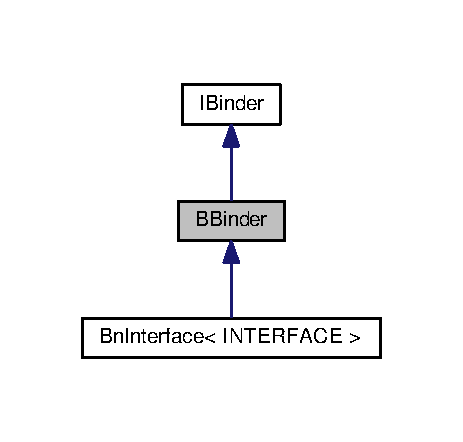
\includegraphics[width=222pt]{classBBinder__inherit__graph}
\end{center}
\end{figure}


Collaboration diagram for B\-Binder\-:
\nopagebreak
\begin{figure}[H]
\begin{center}
\leavevmode
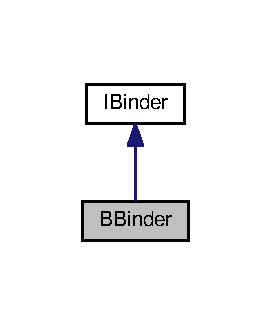
\includegraphics[width=130pt]{classBBinder__coll__graph}
\end{center}
\end{figure}
\subsection*{Public Member Functions}
\begin{DoxyCompactItemize}
\item 
int \hyperlink{classBBinder_a3017278da0f18ac1280f328ac1cab221}{transact} (int code, int $\ast$msg, int $\ast$reply)
\item 
virtual int \hyperlink{classBBinder_addc75a03848c5555aff5a45f08f86898}{on\-Transact} (int, int $\ast$, int $\ast$)
\end{DoxyCompactItemize}


\subsection{Member Function Documentation}
\hypertarget{classBBinder_addc75a03848c5555aff5a45f08f86898}{\index{B\-Binder@{B\-Binder}!on\-Transact@{on\-Transact}}
\index{on\-Transact@{on\-Transact}!BBinder@{B\-Binder}}
\subsubsection[{on\-Transact}]{\setlength{\rightskip}{0pt plus 5cm}virtual int B\-Binder\-::on\-Transact (
\begin{DoxyParamCaption}
\item[{int}]{, }
\item[{int $\ast$}]{, }
\item[{int $\ast$}]{}
\end{DoxyParamCaption}
)\hspace{0.3cm}{\ttfamily [inline]}, {\ttfamily [virtual]}}}\label{classBBinder_addc75a03848c5555aff5a45f08f86898}
\hypertarget{classBBinder_a3017278da0f18ac1280f328ac1cab221}{\index{B\-Binder@{B\-Binder}!transact@{transact}}
\index{transact@{transact}!BBinder@{B\-Binder}}
\subsubsection[{transact}]{\setlength{\rightskip}{0pt plus 5cm}int B\-Binder\-::transact (
\begin{DoxyParamCaption}
\item[{int}]{code, }
\item[{int $\ast$}]{msg, }
\item[{int $\ast$}]{reply}
\end{DoxyParamCaption}
)\hspace{0.3cm}{\ttfamily [inline]}, {\ttfamily [virtual]}}}\label{classBBinder_a3017278da0f18ac1280f328ac1cab221}


Implements \hyperlink{classIBinder_aecaee0fd230aab5cea5b28e0fc88f426}{I\-Binder}.



Here is the call graph for this function\-:
\nopagebreak
\begin{figure}[H]
\begin{center}
\leavevmode
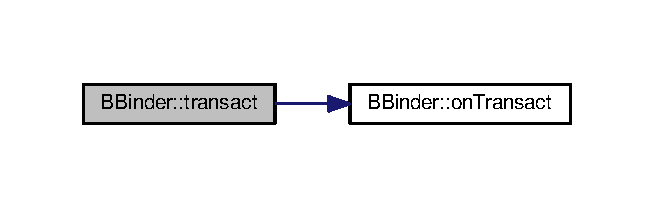
\includegraphics[width=314pt]{classBBinder_a3017278da0f18ac1280f328ac1cab221_cgraph}
\end{center}
\end{figure}




The documentation for this class was generated from the following file\-:\begin{DoxyCompactItemize}
\item 
\hyperlink{binder_8h}{binder.\-h}\end{DoxyCompactItemize}

\hypertarget{classBnInterface}{\section{Bn\-Interface$<$ I\-N\-T\-E\-R\-F\-A\-C\-E $>$ Class Template Reference}
\label{classBnInterface}\index{Bn\-Interface$<$ I\-N\-T\-E\-R\-F\-A\-C\-E $>$@{Bn\-Interface$<$ I\-N\-T\-E\-R\-F\-A\-C\-E $>$}}
}


{\ttfamily \#include $<$binder.\-h$>$}



Inheritance diagram for Bn\-Interface$<$ I\-N\-T\-E\-R\-F\-A\-C\-E $>$\-:
\nopagebreak
\begin{figure}[H]
\begin{center}
\leavevmode
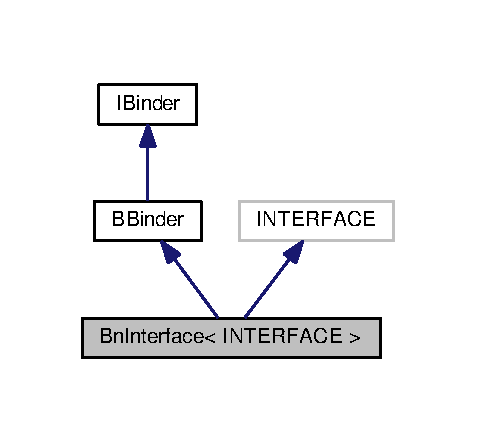
\includegraphics[width=229pt]{classBnInterface__inherit__graph}
\end{center}
\end{figure}


Collaboration diagram for Bn\-Interface$<$ I\-N\-T\-E\-R\-F\-A\-C\-E $>$\-:
\nopagebreak
\begin{figure}[H]
\begin{center}
\leavevmode
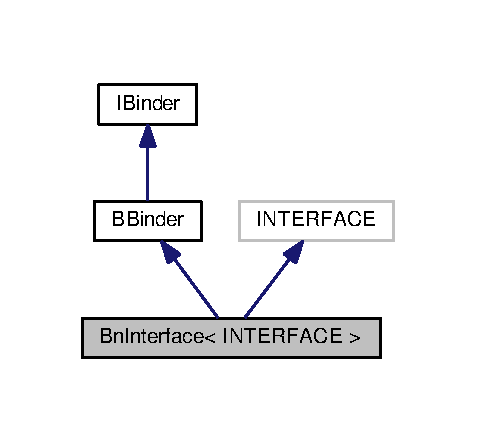
\includegraphics[width=229pt]{classBnInterface__coll__graph}
\end{center}
\end{figure}
\subsection*{Public Member Functions}
\begin{DoxyCompactItemize}
\item 
\hyperlink{classIBinder}{I\-Binder} $\ast$ \hyperlink{classBnInterface_a1562cc058795bdbf837a50ccf1510c1b}{on\-As\-Binder} ()
\item 
int \hyperlink{classBBinder_a3017278da0f18ac1280f328ac1cab221}{transact} (int code, int $\ast$msg, int $\ast$reply)
\item 
virtual int \hyperlink{classBBinder_addc75a03848c5555aff5a45f08f86898}{on\-Transact} (int, int $\ast$, int $\ast$)
\end{DoxyCompactItemize}


\subsection{Member Function Documentation}
\hypertarget{classBnInterface_a1562cc058795bdbf837a50ccf1510c1b}{\index{Bn\-Interface@{Bn\-Interface}!on\-As\-Binder@{on\-As\-Binder}}
\index{on\-As\-Binder@{on\-As\-Binder}!BnInterface@{Bn\-Interface}}
\subsubsection[{on\-As\-Binder}]{\setlength{\rightskip}{0pt plus 5cm}template$<$typename I\-N\-T\-E\-R\-F\-A\-C\-E $>$ {\bf I\-Binder}$\ast$ {\bf Bn\-Interface}$<$ I\-N\-T\-E\-R\-F\-A\-C\-E $>$\-::on\-As\-Binder (
\begin{DoxyParamCaption}
{}
\end{DoxyParamCaption}
)\hspace{0.3cm}{\ttfamily [inline]}}}\label{classBnInterface_a1562cc058795bdbf837a50ccf1510c1b}
\hypertarget{classBBinder_addc75a03848c5555aff5a45f08f86898}{\index{Bn\-Interface@{Bn\-Interface}!on\-Transact@{on\-Transact}}
\index{on\-Transact@{on\-Transact}!BnInterface@{Bn\-Interface}}
\subsubsection[{on\-Transact}]{\setlength{\rightskip}{0pt plus 5cm}virtual int B\-Binder\-::on\-Transact (
\begin{DoxyParamCaption}
\item[{int}]{, }
\item[{int $\ast$}]{, }
\item[{int $\ast$}]{}
\end{DoxyParamCaption}
)\hspace{0.3cm}{\ttfamily [inline]}, {\ttfamily [virtual]}, {\ttfamily [inherited]}}}\label{classBBinder_addc75a03848c5555aff5a45f08f86898}
\hypertarget{classBBinder_a3017278da0f18ac1280f328ac1cab221}{\index{Bn\-Interface@{Bn\-Interface}!transact@{transact}}
\index{transact@{transact}!BnInterface@{Bn\-Interface}}
\subsubsection[{transact}]{\setlength{\rightskip}{0pt plus 5cm}int B\-Binder\-::transact (
\begin{DoxyParamCaption}
\item[{int}]{code, }
\item[{int $\ast$}]{msg, }
\item[{int $\ast$}]{reply}
\end{DoxyParamCaption}
)\hspace{0.3cm}{\ttfamily [inline]}, {\ttfamily [virtual]}, {\ttfamily [inherited]}}}\label{classBBinder_a3017278da0f18ac1280f328ac1cab221}


Implements \hyperlink{classIBinder_aecaee0fd230aab5cea5b28e0fc88f426}{I\-Binder}.



Here is the call graph for this function\-:
\nopagebreak
\begin{figure}[H]
\begin{center}
\leavevmode
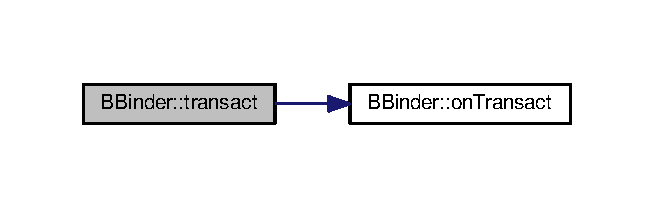
\includegraphics[width=314pt]{classBBinder_a3017278da0f18ac1280f328ac1cab221_cgraph}
\end{center}
\end{figure}




The documentation for this class was generated from the following file\-:\begin{DoxyCompactItemize}
\item 
\hyperlink{binder_8h}{binder.\-h}\end{DoxyCompactItemize}

\hypertarget{classBpBinder}{\section{Bp\-Binder Class Reference}
\label{classBpBinder}\index{Bp\-Binder@{Bp\-Binder}}
}


{\ttfamily \#include $<$binder.\-h$>$}



Inheritance diagram for Bp\-Binder\-:
\nopagebreak
\begin{figure}[H]
\begin{center}
\leavevmode
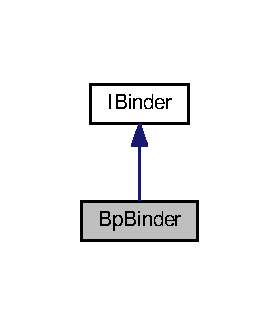
\includegraphics[width=134pt]{classBpBinder__inherit__graph}
\end{center}
\end{figure}


Collaboration diagram for Bp\-Binder\-:
\nopagebreak
\begin{figure}[H]
\begin{center}
\leavevmode
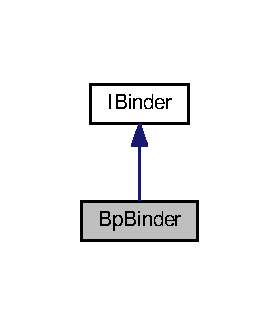
\includegraphics[width=134pt]{classBpBinder__coll__graph}
\end{center}
\end{figure}
\subsection*{Public Member Functions}
\begin{DoxyCompactItemize}
\item 
\hyperlink{classBpBinder_a7e773b3a4a5f65b7645c691e9b25c018}{$\sim$\-Bp\-Binder} ()
\item 
\hyperlink{classBpBinder_a5fc7fa443fe73dbf86cdb33c301563d9}{Bp\-Binder} (int handle)
\item 
int \hyperlink{classBpBinder_a55c5d2af946bce92156a921a6a94a23d}{transact} (int code, int $\ast$msg, int $\ast$reply)
\end{DoxyCompactItemize}
\subsection*{Private Attributes}
\begin{DoxyCompactItemize}
\item 
int \hyperlink{classBpBinder_adab057f2c49454e85f48209499884bd3}{m\-Handle}
\end{DoxyCompactItemize}


\subsection{Constructor \& Destructor Documentation}
\hypertarget{classBpBinder_a7e773b3a4a5f65b7645c691e9b25c018}{\index{Bp\-Binder@{Bp\-Binder}!$\sim$\-Bp\-Binder@{$\sim$\-Bp\-Binder}}
\index{$\sim$\-Bp\-Binder@{$\sim$\-Bp\-Binder}!BpBinder@{Bp\-Binder}}
\subsubsection[{$\sim$\-Bp\-Binder}]{\setlength{\rightskip}{0pt plus 5cm}Bp\-Binder\-::$\sim$\-Bp\-Binder (
\begin{DoxyParamCaption}
{}
\end{DoxyParamCaption}
)\hspace{0.3cm}{\ttfamily [inline]}}}\label{classBpBinder_a7e773b3a4a5f65b7645c691e9b25c018}
\hypertarget{classBpBinder_a5fc7fa443fe73dbf86cdb33c301563d9}{\index{Bp\-Binder@{Bp\-Binder}!Bp\-Binder@{Bp\-Binder}}
\index{Bp\-Binder@{Bp\-Binder}!BpBinder@{Bp\-Binder}}
\subsubsection[{Bp\-Binder}]{\setlength{\rightskip}{0pt plus 5cm}Bp\-Binder\-::\-Bp\-Binder (
\begin{DoxyParamCaption}
\item[{int}]{handle}
\end{DoxyParamCaption}
)\hspace{0.3cm}{\ttfamily [inline]}}}\label{classBpBinder_a5fc7fa443fe73dbf86cdb33c301563d9}


\subsection{Member Function Documentation}
\hypertarget{classBpBinder_a55c5d2af946bce92156a921a6a94a23d}{\index{Bp\-Binder@{Bp\-Binder}!transact@{transact}}
\index{transact@{transact}!BpBinder@{Bp\-Binder}}
\subsubsection[{transact}]{\setlength{\rightskip}{0pt plus 5cm}int Bp\-Binder\-::transact (
\begin{DoxyParamCaption}
\item[{int}]{code, }
\item[{int $\ast$}]{msg, }
\item[{int $\ast$}]{reply}
\end{DoxyParamCaption}
)\hspace{0.3cm}{\ttfamily [inline]}, {\ttfamily [virtual]}}}\label{classBpBinder_a55c5d2af946bce92156a921a6a94a23d}


Implements \hyperlink{classIBinder_aecaee0fd230aab5cea5b28e0fc88f426}{I\-Binder}.



Here is the call graph for this function\-:
\nopagebreak
\begin{figure}[H]
\begin{center}
\leavevmode
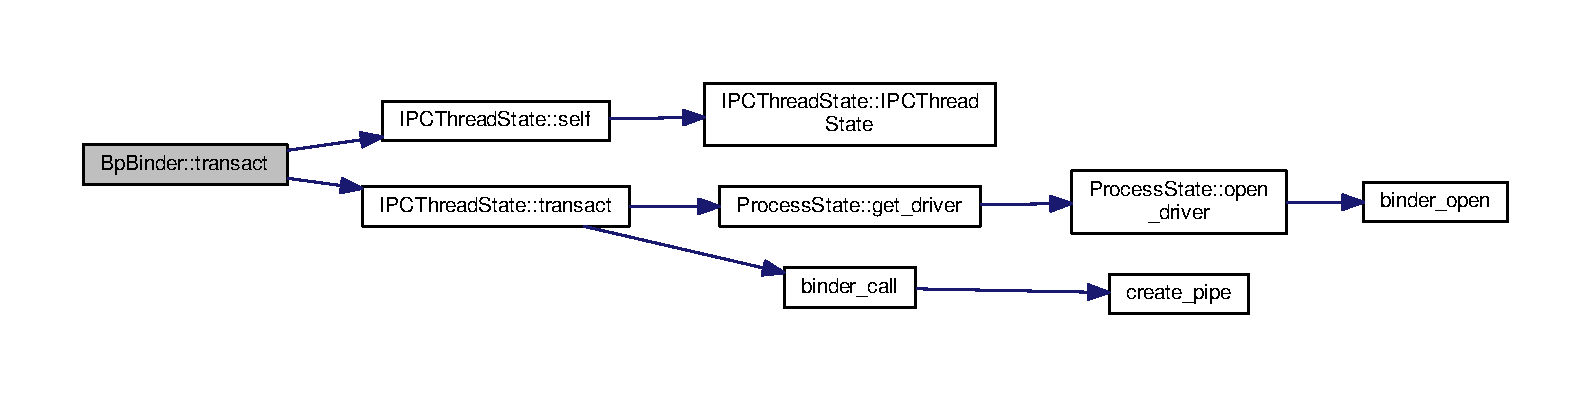
\includegraphics[width=350pt]{classBpBinder_a55c5d2af946bce92156a921a6a94a23d_cgraph}
\end{center}
\end{figure}




\subsection{Member Data Documentation}
\hypertarget{classBpBinder_adab057f2c49454e85f48209499884bd3}{\index{Bp\-Binder@{Bp\-Binder}!m\-Handle@{m\-Handle}}
\index{m\-Handle@{m\-Handle}!BpBinder@{Bp\-Binder}}
\subsubsection[{m\-Handle}]{\setlength{\rightskip}{0pt plus 5cm}int Bp\-Binder\-::m\-Handle\hspace{0.3cm}{\ttfamily [private]}}}\label{classBpBinder_adab057f2c49454e85f48209499884bd3}


The documentation for this class was generated from the following file\-:\begin{DoxyCompactItemize}
\item 
\hyperlink{binder_8h}{binder.\-h}\end{DoxyCompactItemize}

\hypertarget{classBpInterface}{\section{Bp\-Interface$<$ I\-N\-T\-E\-R\-F\-A\-C\-E $>$ Class Template Reference}
\label{classBpInterface}\index{Bp\-Interface$<$ I\-N\-T\-E\-R\-F\-A\-C\-E $>$@{Bp\-Interface$<$ I\-N\-T\-E\-R\-F\-A\-C\-E $>$}}
}


{\ttfamily \#include $<$binder.\-h$>$}



Inheritance diagram for Bp\-Interface$<$ I\-N\-T\-E\-R\-F\-A\-C\-E $>$\-:
\nopagebreak
\begin{figure}[H]
\begin{center}
\leavevmode
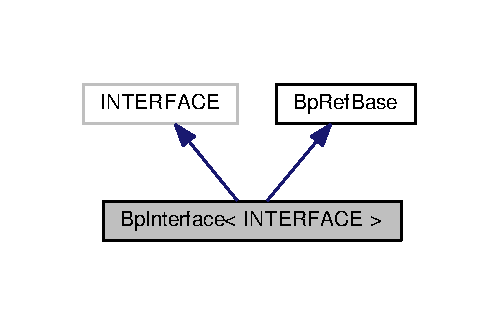
\includegraphics[width=239pt]{classBpInterface__inherit__graph}
\end{center}
\end{figure}


Collaboration diagram for Bp\-Interface$<$ I\-N\-T\-E\-R\-F\-A\-C\-E $>$\-:
\nopagebreak
\begin{figure}[H]
\begin{center}
\leavevmode
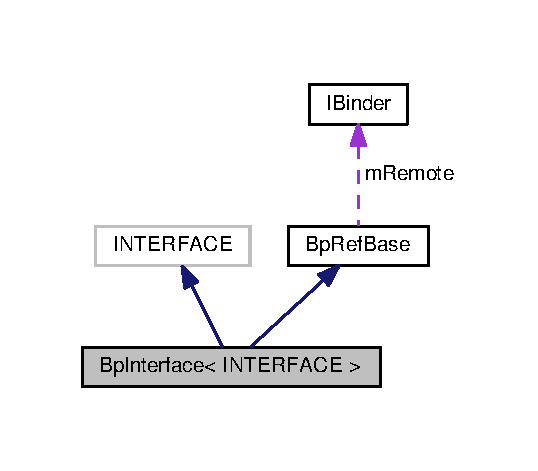
\includegraphics[width=258pt]{classBpInterface__coll__graph}
\end{center}
\end{figure}
\subsection*{Public Member Functions}
\begin{DoxyCompactItemize}
\item 
\hyperlink{classBpInterface_ab9ef538cb62a632785f91d5ece2dbdb0}{Bp\-Interface} (\hyperlink{classIBinder}{I\-Binder} $\ast$p)
\item 
\hyperlink{classIBinder}{I\-Binder} $\ast$ \hyperlink{classBpInterface_a86ad98fefa1cc283be87c8a501f587b8}{on\-As\-Binder} ()
\item 
\hyperlink{classIBinder}{I\-Binder} $\ast$ \hyperlink{classBpRefBase_ac52fd0b3fb7dbf09140993c73a6c3a3e}{remote} ()
\end{DoxyCompactItemize}


\subsection{Constructor \& Destructor Documentation}
\hypertarget{classBpInterface_ab9ef538cb62a632785f91d5ece2dbdb0}{\index{Bp\-Interface@{Bp\-Interface}!Bp\-Interface@{Bp\-Interface}}
\index{Bp\-Interface@{Bp\-Interface}!BpInterface@{Bp\-Interface}}
\subsubsection[{Bp\-Interface}]{\setlength{\rightskip}{0pt plus 5cm}template$<$typename I\-N\-T\-E\-R\-F\-A\-C\-E $>$ {\bf Bp\-Interface}$<$ I\-N\-T\-E\-R\-F\-A\-C\-E $>$\-::{\bf Bp\-Interface} (
\begin{DoxyParamCaption}
\item[{{\bf I\-Binder} $\ast$}]{p}
\end{DoxyParamCaption}
)\hspace{0.3cm}{\ttfamily [inline]}}}\label{classBpInterface_ab9ef538cb62a632785f91d5ece2dbdb0}


\subsection{Member Function Documentation}
\hypertarget{classBpInterface_a86ad98fefa1cc283be87c8a501f587b8}{\index{Bp\-Interface@{Bp\-Interface}!on\-As\-Binder@{on\-As\-Binder}}
\index{on\-As\-Binder@{on\-As\-Binder}!BpInterface@{Bp\-Interface}}
\subsubsection[{on\-As\-Binder}]{\setlength{\rightskip}{0pt plus 5cm}template$<$typename I\-N\-T\-E\-R\-F\-A\-C\-E $>$ {\bf I\-Binder}$\ast$ {\bf Bp\-Interface}$<$ I\-N\-T\-E\-R\-F\-A\-C\-E $>$\-::on\-As\-Binder (
\begin{DoxyParamCaption}
{}
\end{DoxyParamCaption}
)\hspace{0.3cm}{\ttfamily [inline]}}}\label{classBpInterface_a86ad98fefa1cc283be87c8a501f587b8}


Here is the call graph for this function\-:
\nopagebreak
\begin{figure}[H]
\begin{center}
\leavevmode
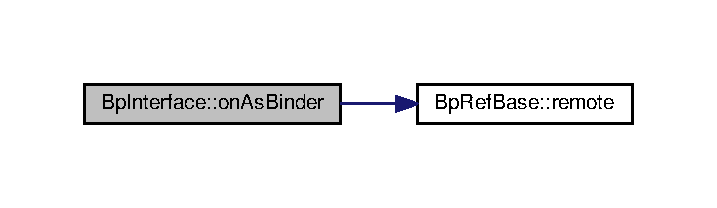
\includegraphics[width=344pt]{classBpInterface_a86ad98fefa1cc283be87c8a501f587b8_cgraph}
\end{center}
\end{figure}


\hypertarget{classBpRefBase_ac52fd0b3fb7dbf09140993c73a6c3a3e}{\index{Bp\-Interface@{Bp\-Interface}!remote@{remote}}
\index{remote@{remote}!BpInterface@{Bp\-Interface}}
\subsubsection[{remote}]{\setlength{\rightskip}{0pt plus 5cm}{\bf I\-Binder}$\ast$ Bp\-Ref\-Base\-::remote (
\begin{DoxyParamCaption}
{}
\end{DoxyParamCaption}
)\hspace{0.3cm}{\ttfamily [inline]}, {\ttfamily [inherited]}}}\label{classBpRefBase_ac52fd0b3fb7dbf09140993c73a6c3a3e}


The documentation for this class was generated from the following file\-:\begin{DoxyCompactItemize}
\item 
\hyperlink{binder_8h}{binder.\-h}\end{DoxyCompactItemize}

\hypertarget{classBpRefBase}{\section{Bp\-Ref\-Base Class Reference}
\label{classBpRefBase}\index{Bp\-Ref\-Base@{Bp\-Ref\-Base}}
}


{\ttfamily \#include $<$binder.\-h$>$}



Inheritance diagram for Bp\-Ref\-Base\-:
\nopagebreak
\begin{figure}[H]
\begin{center}
\leavevmode
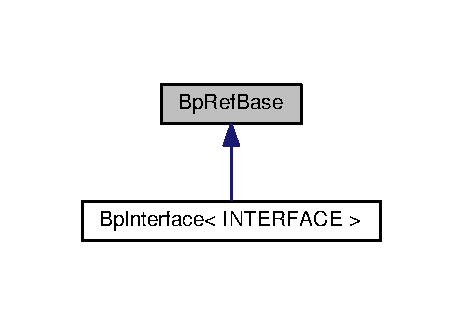
\includegraphics[width=222pt]{classBpRefBase__inherit__graph}
\end{center}
\end{figure}


Collaboration diagram for Bp\-Ref\-Base\-:
\nopagebreak
\begin{figure}[H]
\begin{center}
\leavevmode
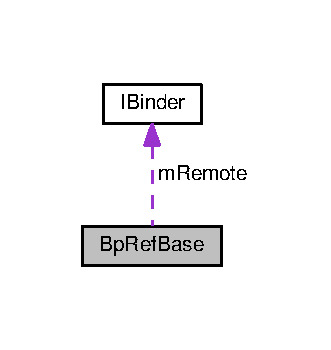
\includegraphics[width=159pt]{classBpRefBase__coll__graph}
\end{center}
\end{figure}
\subsection*{Public Member Functions}
\begin{DoxyCompactItemize}
\item 
\hyperlink{classBpRefBase_aef592ef9a6af0dfe2101da969c5f5ab0}{Bp\-Ref\-Base} (\hyperlink{classIBinder}{I\-Binder} $\ast$p)
\item 
\hyperlink{classIBinder}{I\-Binder} $\ast$ \hyperlink{classBpRefBase_ac52fd0b3fb7dbf09140993c73a6c3a3e}{remote} ()
\end{DoxyCompactItemize}
\subsection*{Private Attributes}
\begin{DoxyCompactItemize}
\item 
\hyperlink{classIBinder}{I\-Binder} $\ast$ \hyperlink{classBpRefBase_a92cbe99f30ddf5e4f8a73102f5c9ebb0}{m\-Remote}
\end{DoxyCompactItemize}


\subsection{Constructor \& Destructor Documentation}
\hypertarget{classBpRefBase_aef592ef9a6af0dfe2101da969c5f5ab0}{\index{Bp\-Ref\-Base@{Bp\-Ref\-Base}!Bp\-Ref\-Base@{Bp\-Ref\-Base}}
\index{Bp\-Ref\-Base@{Bp\-Ref\-Base}!BpRefBase@{Bp\-Ref\-Base}}
\subsubsection[{Bp\-Ref\-Base}]{\setlength{\rightskip}{0pt plus 5cm}Bp\-Ref\-Base\-::\-Bp\-Ref\-Base (
\begin{DoxyParamCaption}
\item[{{\bf I\-Binder} $\ast$}]{p}
\end{DoxyParamCaption}
)\hspace{0.3cm}{\ttfamily [inline]}}}\label{classBpRefBase_aef592ef9a6af0dfe2101da969c5f5ab0}


\subsection{Member Function Documentation}
\hypertarget{classBpRefBase_ac52fd0b3fb7dbf09140993c73a6c3a3e}{\index{Bp\-Ref\-Base@{Bp\-Ref\-Base}!remote@{remote}}
\index{remote@{remote}!BpRefBase@{Bp\-Ref\-Base}}
\subsubsection[{remote}]{\setlength{\rightskip}{0pt plus 5cm}{\bf I\-Binder}$\ast$ Bp\-Ref\-Base\-::remote (
\begin{DoxyParamCaption}
{}
\end{DoxyParamCaption}
)\hspace{0.3cm}{\ttfamily [inline]}}}\label{classBpRefBase_ac52fd0b3fb7dbf09140993c73a6c3a3e}


\subsection{Member Data Documentation}
\hypertarget{classBpRefBase_a92cbe99f30ddf5e4f8a73102f5c9ebb0}{\index{Bp\-Ref\-Base@{Bp\-Ref\-Base}!m\-Remote@{m\-Remote}}
\index{m\-Remote@{m\-Remote}!BpRefBase@{Bp\-Ref\-Base}}
\subsubsection[{m\-Remote}]{\setlength{\rightskip}{0pt plus 5cm}{\bf I\-Binder}$\ast$ Bp\-Ref\-Base\-::m\-Remote\hspace{0.3cm}{\ttfamily [private]}}}\label{classBpRefBase_a92cbe99f30ddf5e4f8a73102f5c9ebb0}


The documentation for this class was generated from the following file\-:\begin{DoxyCompactItemize}
\item 
\hyperlink{binder_8h}{binder.\-h}\end{DoxyCompactItemize}

\hypertarget{classIBinder}{\section{I\-Binder Class Reference}
\label{classIBinder}\index{I\-Binder@{I\-Binder}}
}


{\ttfamily \#include $<$binder.\-h$>$}



Inheritance diagram for I\-Binder\-:
\nopagebreak
\begin{figure}[H]
\begin{center}
\leavevmode
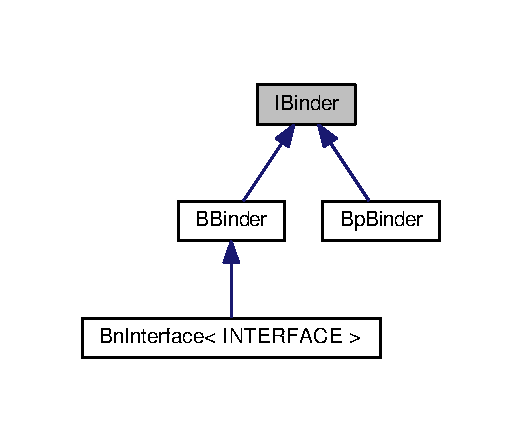
\includegraphics[width=251pt]{classIBinder__inherit__graph}
\end{center}
\end{figure}
\subsection*{Public Member Functions}
\begin{DoxyCompactItemize}
\item 
virtual int \hyperlink{classIBinder_aecaee0fd230aab5cea5b28e0fc88f426}{transact} (int code, int $\ast$msg, int $\ast$reply)=0
\item 
virtual \hyperlink{classIBinder_afa6dfa2e8c000de5d6aabc61f451ba02}{$\sim$\-I\-Binder} ()
\end{DoxyCompactItemize}


\subsection{Constructor \& Destructor Documentation}
\hypertarget{classIBinder_afa6dfa2e8c000de5d6aabc61f451ba02}{\index{I\-Binder@{I\-Binder}!$\sim$\-I\-Binder@{$\sim$\-I\-Binder}}
\index{$\sim$\-I\-Binder@{$\sim$\-I\-Binder}!IBinder@{I\-Binder}}
\subsubsection[{$\sim$\-I\-Binder}]{\setlength{\rightskip}{0pt plus 5cm}virtual I\-Binder\-::$\sim$\-I\-Binder (
\begin{DoxyParamCaption}
{}
\end{DoxyParamCaption}
)\hspace{0.3cm}{\ttfamily [inline]}, {\ttfamily [virtual]}}}\label{classIBinder_afa6dfa2e8c000de5d6aabc61f451ba02}


\subsection{Member Function Documentation}
\hypertarget{classIBinder_aecaee0fd230aab5cea5b28e0fc88f426}{\index{I\-Binder@{I\-Binder}!transact@{transact}}
\index{transact@{transact}!IBinder@{I\-Binder}}
\subsubsection[{transact}]{\setlength{\rightskip}{0pt plus 5cm}virtual int I\-Binder\-::transact (
\begin{DoxyParamCaption}
\item[{int}]{code, }
\item[{int $\ast$}]{msg, }
\item[{int $\ast$}]{reply}
\end{DoxyParamCaption}
)\hspace{0.3cm}{\ttfamily [pure virtual]}}}\label{classIBinder_aecaee0fd230aab5cea5b28e0fc88f426}


Implemented in \hyperlink{classBpBinder_a55c5d2af946bce92156a921a6a94a23d}{Bp\-Binder}, and \hyperlink{classBBinder_a3017278da0f18ac1280f328ac1cab221}{B\-Binder}.



The documentation for this class was generated from the following file\-:\begin{DoxyCompactItemize}
\item 
\hyperlink{binder_8h}{binder.\-h}\end{DoxyCompactItemize}

\hypertarget{classIInterface}{\section{I\-Interface Class Reference}
\label{classIInterface}\index{I\-Interface@{I\-Interface}}
}


{\ttfamily \#include $<$binder.\-h$>$}



Inheritance diagram for I\-Interface\-:
\nopagebreak
\begin{figure}[H]
\begin{center}
\leavevmode
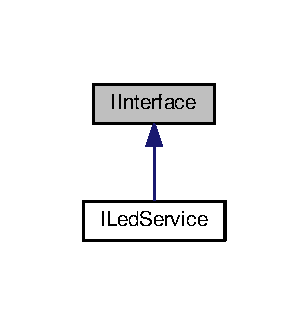
\includegraphics[width=148pt]{classIInterface__inherit__graph}
\end{center}
\end{figure}
\subsection*{Public Member Functions}
\begin{DoxyCompactItemize}
\item 
\hyperlink{classIBinder}{I\-Binder} $\ast$ \hyperlink{classIInterface_ab440604e1acbdcae2c7d652a8e10d9bc}{as\-Binder} ()
\item 
virtual \hyperlink{classIBinder}{I\-Binder} $\ast$ \hyperlink{classIInterface_a7fc01137c48beca773b32e182c13d6dc}{on\-As\-Binder} ()=0
\end{DoxyCompactItemize}


\subsection{Member Function Documentation}
\hypertarget{classIInterface_ab440604e1acbdcae2c7d652a8e10d9bc}{\index{I\-Interface@{I\-Interface}!as\-Binder@{as\-Binder}}
\index{as\-Binder@{as\-Binder}!IInterface@{I\-Interface}}
\subsubsection[{as\-Binder}]{\setlength{\rightskip}{0pt plus 5cm}{\bf I\-Binder}$\ast$ I\-Interface\-::as\-Binder (
\begin{DoxyParamCaption}
{}
\end{DoxyParamCaption}
)\hspace{0.3cm}{\ttfamily [inline]}}}\label{classIInterface_ab440604e1acbdcae2c7d652a8e10d9bc}


Here is the call graph for this function\-:
\nopagebreak
\begin{figure}[H]
\begin{center}
\leavevmode
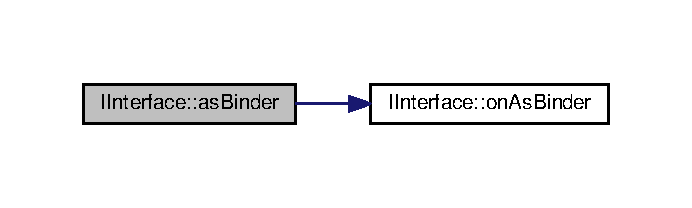
\includegraphics[width=332pt]{classIInterface_ab440604e1acbdcae2c7d652a8e10d9bc_cgraph}
\end{center}
\end{figure}


\hypertarget{classIInterface_a7fc01137c48beca773b32e182c13d6dc}{\index{I\-Interface@{I\-Interface}!on\-As\-Binder@{on\-As\-Binder}}
\index{on\-As\-Binder@{on\-As\-Binder}!IInterface@{I\-Interface}}
\subsubsection[{on\-As\-Binder}]{\setlength{\rightskip}{0pt plus 5cm}virtual {\bf I\-Binder}$\ast$ I\-Interface\-::on\-As\-Binder (
\begin{DoxyParamCaption}
{}
\end{DoxyParamCaption}
)\hspace{0.3cm}{\ttfamily [pure virtual]}}}\label{classIInterface_a7fc01137c48beca773b32e182c13d6dc}


The documentation for this class was generated from the following file\-:\begin{DoxyCompactItemize}
\item 
\hyperlink{binder_8h}{binder.\-h}\end{DoxyCompactItemize}

\hypertarget{classILedService}{\section{I\-Led\-Service Class Reference}
\label{classILedService}\index{I\-Led\-Service@{I\-Led\-Service}}
}


{\ttfamily \#include $<$binder.\-h$>$}



Inheritance diagram for I\-Led\-Service\-:
\nopagebreak
\begin{figure}[H]
\begin{center}
\leavevmode
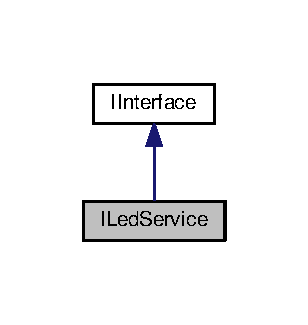
\includegraphics[width=148pt]{classILedService__inherit__graph}
\end{center}
\end{figure}


Collaboration diagram for I\-Led\-Service\-:
\nopagebreak
\begin{figure}[H]
\begin{center}
\leavevmode
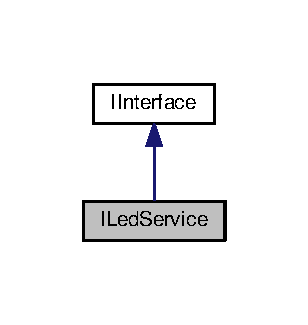
\includegraphics[width=148pt]{classILedService__coll__graph}
\end{center}
\end{figure}
\subsection*{Public Member Functions}
\begin{DoxyCompactItemize}
\item 
virtual void \hyperlink{classILedService_ae6cd7ce85f6f28bcb2a61509ca3c54cd}{led\-On} ()=0
\item 
virtual void \hyperlink{classILedService_a799ed43550560099c81f13bf9e2dae09}{led\-Off} ()=0
\item 
virtual \hyperlink{classILedService_a2ead1c2f6ad19c4385e52b5bfaeb3a9c}{$\sim$\-I\-Led\-Service} ()
\item 
\hyperlink{classILedService_ad4b3c31ad0ca92dd42b0f01e48ab83ed}{D\-E\-C\-L\-A\-R\-E\-\_\-\-M\-E\-T\-A\-\_\-\-I\-N\-T\-E\-R\-F\-A\-C\-E} (Led\-Service)
\item 
\hyperlink{classIBinder}{I\-Binder} $\ast$ \hyperlink{classIInterface_ab440604e1acbdcae2c7d652a8e10d9bc}{as\-Binder} ()
\item 
virtual \hyperlink{classIBinder}{I\-Binder} $\ast$ \hyperlink{classIInterface_a7fc01137c48beca773b32e182c13d6dc}{on\-As\-Binder} ()=0
\end{DoxyCompactItemize}


\subsection{Constructor \& Destructor Documentation}
\hypertarget{classILedService_a2ead1c2f6ad19c4385e52b5bfaeb3a9c}{\index{I\-Led\-Service@{I\-Led\-Service}!$\sim$\-I\-Led\-Service@{$\sim$\-I\-Led\-Service}}
\index{$\sim$\-I\-Led\-Service@{$\sim$\-I\-Led\-Service}!ILedService@{I\-Led\-Service}}
\subsubsection[{$\sim$\-I\-Led\-Service}]{\setlength{\rightskip}{0pt plus 5cm}virtual I\-Led\-Service\-::$\sim$\-I\-Led\-Service (
\begin{DoxyParamCaption}
{}
\end{DoxyParamCaption}
)\hspace{0.3cm}{\ttfamily [inline]}, {\ttfamily [virtual]}}}\label{classILedService_a2ead1c2f6ad19c4385e52b5bfaeb3a9c}


\subsection{Member Function Documentation}
\hypertarget{classIInterface_ab440604e1acbdcae2c7d652a8e10d9bc}{\index{I\-Led\-Service@{I\-Led\-Service}!as\-Binder@{as\-Binder}}
\index{as\-Binder@{as\-Binder}!ILedService@{I\-Led\-Service}}
\subsubsection[{as\-Binder}]{\setlength{\rightskip}{0pt plus 5cm}{\bf I\-Binder}$\ast$ I\-Interface\-::as\-Binder (
\begin{DoxyParamCaption}
{}
\end{DoxyParamCaption}
)\hspace{0.3cm}{\ttfamily [inline]}, {\ttfamily [inherited]}}}\label{classIInterface_ab440604e1acbdcae2c7d652a8e10d9bc}


Here is the call graph for this function\-:
\nopagebreak
\begin{figure}[H]
\begin{center}
\leavevmode
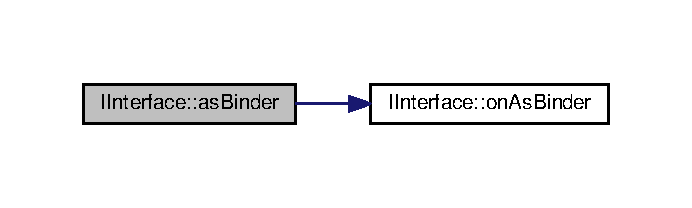
\includegraphics[width=332pt]{classIInterface_ab440604e1acbdcae2c7d652a8e10d9bc_cgraph}
\end{center}
\end{figure}


\hypertarget{classILedService_ad4b3c31ad0ca92dd42b0f01e48ab83ed}{\index{I\-Led\-Service@{I\-Led\-Service}!D\-E\-C\-L\-A\-R\-E\-\_\-\-M\-E\-T\-A\-\_\-\-I\-N\-T\-E\-R\-F\-A\-C\-E@{D\-E\-C\-L\-A\-R\-E\-\_\-\-M\-E\-T\-A\-\_\-\-I\-N\-T\-E\-R\-F\-A\-C\-E}}
\index{D\-E\-C\-L\-A\-R\-E\-\_\-\-M\-E\-T\-A\-\_\-\-I\-N\-T\-E\-R\-F\-A\-C\-E@{D\-E\-C\-L\-A\-R\-E\-\_\-\-M\-E\-T\-A\-\_\-\-I\-N\-T\-E\-R\-F\-A\-C\-E}!ILedService@{I\-Led\-Service}}
\subsubsection[{D\-E\-C\-L\-A\-R\-E\-\_\-\-M\-E\-T\-A\-\_\-\-I\-N\-T\-E\-R\-F\-A\-C\-E}]{\setlength{\rightskip}{0pt plus 5cm}I\-Led\-Service\-::\-D\-E\-C\-L\-A\-R\-E\-\_\-\-M\-E\-T\-A\-\_\-\-I\-N\-T\-E\-R\-F\-A\-C\-E (
\begin{DoxyParamCaption}
\item[{Led\-Service}]{}
\end{DoxyParamCaption}
)}}\label{classILedService_ad4b3c31ad0ca92dd42b0f01e48ab83ed}
\hypertarget{classILedService_a799ed43550560099c81f13bf9e2dae09}{\index{I\-Led\-Service@{I\-Led\-Service}!led\-Off@{led\-Off}}
\index{led\-Off@{led\-Off}!ILedService@{I\-Led\-Service}}
\subsubsection[{led\-Off}]{\setlength{\rightskip}{0pt plus 5cm}virtual void I\-Led\-Service\-::led\-Off (
\begin{DoxyParamCaption}
{}
\end{DoxyParamCaption}
)\hspace{0.3cm}{\ttfamily [pure virtual]}}}\label{classILedService_a799ed43550560099c81f13bf9e2dae09}
\hypertarget{classILedService_ae6cd7ce85f6f28bcb2a61509ca3c54cd}{\index{I\-Led\-Service@{I\-Led\-Service}!led\-On@{led\-On}}
\index{led\-On@{led\-On}!ILedService@{I\-Led\-Service}}
\subsubsection[{led\-On}]{\setlength{\rightskip}{0pt plus 5cm}virtual void I\-Led\-Service\-::led\-On (
\begin{DoxyParamCaption}
{}
\end{DoxyParamCaption}
)\hspace{0.3cm}{\ttfamily [pure virtual]}}}\label{classILedService_ae6cd7ce85f6f28bcb2a61509ca3c54cd}
\hypertarget{classIInterface_a7fc01137c48beca773b32e182c13d6dc}{\index{I\-Led\-Service@{I\-Led\-Service}!on\-As\-Binder@{on\-As\-Binder}}
\index{on\-As\-Binder@{on\-As\-Binder}!ILedService@{I\-Led\-Service}}
\subsubsection[{on\-As\-Binder}]{\setlength{\rightskip}{0pt plus 5cm}virtual {\bf I\-Binder}$\ast$ I\-Interface\-::on\-As\-Binder (
\begin{DoxyParamCaption}
{}
\end{DoxyParamCaption}
)\hspace{0.3cm}{\ttfamily [pure virtual]}, {\ttfamily [inherited]}}}\label{classIInterface_a7fc01137c48beca773b32e182c13d6dc}


The documentation for this class was generated from the following file\-:\begin{DoxyCompactItemize}
\item 
\hyperlink{binder_8h}{binder.\-h}\end{DoxyCompactItemize}

\hypertarget{classIPCThreadState}{\section{I\-P\-C\-Thread\-State Class Reference}
\label{classIPCThreadState}\index{I\-P\-C\-Thread\-State@{I\-P\-C\-Thread\-State}}
}


{\ttfamily \#include $<$binder.\-h$>$}



Collaboration diagram for I\-P\-C\-Thread\-State\-:
\nopagebreak
\begin{figure}[H]
\begin{center}
\leavevmode
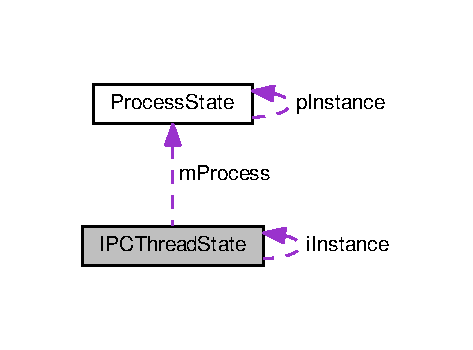
\includegraphics[width=227pt]{classIPCThreadState__coll__graph}
\end{center}
\end{figure}
\subsection*{Public Member Functions}
\begin{DoxyCompactItemize}
\item 
int \hyperlink{classIPCThreadState_a12423983ca5df01ecb79163ea3e0df82}{transact} (int handle, int code, int $\ast$msg, int $\ast$reply)
\item 
void \hyperlink{classIPCThreadState_a68fd78989dbd0ac468b6f9f0cd17b5a8}{join\-Thread\-Pool} ()
\end{DoxyCompactItemize}
\subsection*{Static Public Member Functions}
\begin{DoxyCompactItemize}
\item 
static \hyperlink{classIPCThreadState}{I\-P\-C\-Thread\-State} $\ast$ \hyperlink{classIPCThreadState_a42c7daa79fc1364b3bd3ac8b0920bf0e}{self} ()
\item 
static int \hyperlink{classIPCThreadState_a37c4e27f1770cc5ca7ebd8ed330b4438}{my\-\_\-handler} (int code, int msg, int $\ast$reply)
\end{DoxyCompactItemize}
\subsection*{Private Member Functions}
\begin{DoxyCompactItemize}
\item 
\hyperlink{classIPCThreadState_a6e1a9d9bc01c877747ecae8df73bd14e}{I\-P\-C\-Thread\-State} ()
\item 
\hyperlink{classIPCThreadState_a368b35eb534b0b49e5c0b522d98a0a6d}{I\-P\-C\-Thread\-State} (const \hyperlink{classIPCThreadState}{I\-P\-C\-Thread\-State} $\ast$i)
\item 
\hyperlink{classIPCThreadState}{I\-P\-C\-Thread\-State} \& \hyperlink{classIPCThreadState_a4f68d05d2665e30b2d43479feba7f944}{operator=} (const \hyperlink{classIPCThreadState}{I\-P\-C\-Thread\-State} $\ast$i)
\end{DoxyCompactItemize}
\subsection*{Private Attributes}
\begin{DoxyCompactItemize}
\item 
\hyperlink{classProcessState}{Process\-State} $\ast$ \hyperlink{classIPCThreadState_aefae3c0f96244ce87f9289defee13b54}{m\-Process}
\end{DoxyCompactItemize}
\subsection*{Static Private Attributes}
\begin{DoxyCompactItemize}
\item 
static \hyperlink{classIPCThreadState}{I\-P\-C\-Thread\-State} $\ast$ \hyperlink{classIPCThreadState_a54fefc86880e0e140d40e9aa7247cc47}{i\-Instance} = 0
\end{DoxyCompactItemize}


\subsection{Constructor \& Destructor Documentation}
\hypertarget{classIPCThreadState_a6e1a9d9bc01c877747ecae8df73bd14e}{\index{I\-P\-C\-Thread\-State@{I\-P\-C\-Thread\-State}!I\-P\-C\-Thread\-State@{I\-P\-C\-Thread\-State}}
\index{I\-P\-C\-Thread\-State@{I\-P\-C\-Thread\-State}!IPCThreadState@{I\-P\-C\-Thread\-State}}
\subsubsection[{I\-P\-C\-Thread\-State}]{\setlength{\rightskip}{0pt plus 5cm}I\-P\-C\-Thread\-State\-::\-I\-P\-C\-Thread\-State (
\begin{DoxyParamCaption}
{}
\end{DoxyParamCaption}
)\hspace{0.3cm}{\ttfamily [inline]}, {\ttfamily [private]}}}\label{classIPCThreadState_a6e1a9d9bc01c877747ecae8df73bd14e}
\hypertarget{classIPCThreadState_a368b35eb534b0b49e5c0b522d98a0a6d}{\index{I\-P\-C\-Thread\-State@{I\-P\-C\-Thread\-State}!I\-P\-C\-Thread\-State@{I\-P\-C\-Thread\-State}}
\index{I\-P\-C\-Thread\-State@{I\-P\-C\-Thread\-State}!IPCThreadState@{I\-P\-C\-Thread\-State}}
\subsubsection[{I\-P\-C\-Thread\-State}]{\setlength{\rightskip}{0pt plus 5cm}I\-P\-C\-Thread\-State\-::\-I\-P\-C\-Thread\-State (
\begin{DoxyParamCaption}
\item[{const {\bf I\-P\-C\-Thread\-State} $\ast$}]{i}
\end{DoxyParamCaption}
)\hspace{0.3cm}{\ttfamily [private]}}}\label{classIPCThreadState_a368b35eb534b0b49e5c0b522d98a0a6d}


\subsection{Member Function Documentation}
\hypertarget{classIPCThreadState_a68fd78989dbd0ac468b6f9f0cd17b5a8}{\index{I\-P\-C\-Thread\-State@{I\-P\-C\-Thread\-State}!join\-Thread\-Pool@{join\-Thread\-Pool}}
\index{join\-Thread\-Pool@{join\-Thread\-Pool}!IPCThreadState@{I\-P\-C\-Thread\-State}}
\subsubsection[{join\-Thread\-Pool}]{\setlength{\rightskip}{0pt plus 5cm}void I\-P\-C\-Thread\-State\-::join\-Thread\-Pool (
\begin{DoxyParamCaption}
{}
\end{DoxyParamCaption}
)\hspace{0.3cm}{\ttfamily [inline]}}}\label{classIPCThreadState_a68fd78989dbd0ac468b6f9f0cd17b5a8}


Here is the call graph for this function\-:
\nopagebreak
\begin{figure}[H]
\begin{center}
\leavevmode
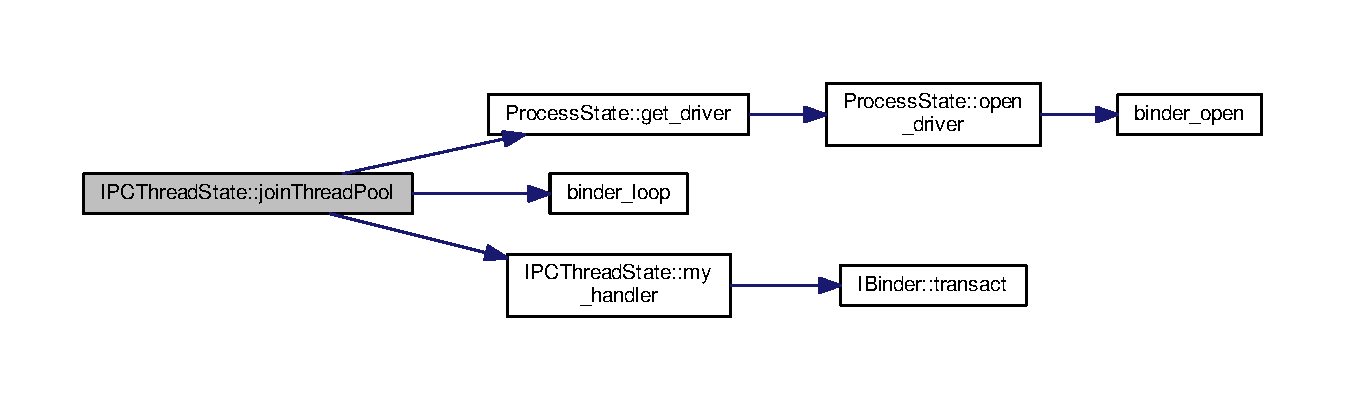
\includegraphics[width=350pt]{classIPCThreadState_a68fd78989dbd0ac468b6f9f0cd17b5a8_cgraph}
\end{center}
\end{figure}


\hypertarget{classIPCThreadState_a37c4e27f1770cc5ca7ebd8ed330b4438}{\index{I\-P\-C\-Thread\-State@{I\-P\-C\-Thread\-State}!my\-\_\-handler@{my\-\_\-handler}}
\index{my\-\_\-handler@{my\-\_\-handler}!IPCThreadState@{I\-P\-C\-Thread\-State}}
\subsubsection[{my\-\_\-handler}]{\setlength{\rightskip}{0pt plus 5cm}static int I\-P\-C\-Thread\-State\-::my\-\_\-handler (
\begin{DoxyParamCaption}
\item[{int}]{code, }
\item[{int}]{msg, }
\item[{int $\ast$}]{reply}
\end{DoxyParamCaption}
)\hspace{0.3cm}{\ttfamily [inline]}, {\ttfamily [static]}}}\label{classIPCThreadState_a37c4e27f1770cc5ca7ebd8ed330b4438}


Here is the call graph for this function\-:
\nopagebreak
\begin{figure}[H]
\begin{center}
\leavevmode
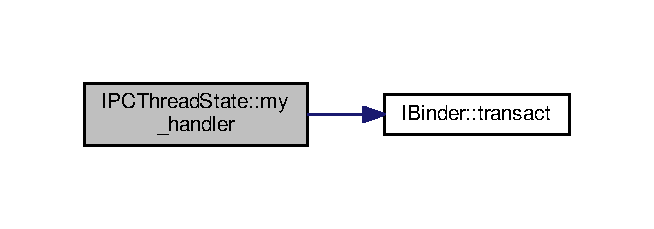
\includegraphics[width=314pt]{classIPCThreadState_a37c4e27f1770cc5ca7ebd8ed330b4438_cgraph}
\end{center}
\end{figure}


\hypertarget{classIPCThreadState_a4f68d05d2665e30b2d43479feba7f944}{\index{I\-P\-C\-Thread\-State@{I\-P\-C\-Thread\-State}!operator=@{operator=}}
\index{operator=@{operator=}!IPCThreadState@{I\-P\-C\-Thread\-State}}
\subsubsection[{operator=}]{\setlength{\rightskip}{0pt plus 5cm}{\bf I\-P\-C\-Thread\-State}\& I\-P\-C\-Thread\-State\-::operator= (
\begin{DoxyParamCaption}
\item[{const {\bf I\-P\-C\-Thread\-State} $\ast$}]{i}
\end{DoxyParamCaption}
)\hspace{0.3cm}{\ttfamily [private]}}}\label{classIPCThreadState_a4f68d05d2665e30b2d43479feba7f944}
\hypertarget{classIPCThreadState_a42c7daa79fc1364b3bd3ac8b0920bf0e}{\index{I\-P\-C\-Thread\-State@{I\-P\-C\-Thread\-State}!self@{self}}
\index{self@{self}!IPCThreadState@{I\-P\-C\-Thread\-State}}
\subsubsection[{self}]{\setlength{\rightskip}{0pt plus 5cm}static {\bf I\-P\-C\-Thread\-State}$\ast$ I\-P\-C\-Thread\-State\-::self (
\begin{DoxyParamCaption}
{}
\end{DoxyParamCaption}
)\hspace{0.3cm}{\ttfamily [inline]}, {\ttfamily [static]}}}\label{classIPCThreadState_a42c7daa79fc1364b3bd3ac8b0920bf0e}


Here is the call graph for this function\-:
\nopagebreak
\begin{figure}[H]
\begin{center}
\leavevmode

\includegraphics[width=350pt]{classIPCThreadState_a42c7daa79fc1364b3bd3ac8b0920bf0e_cgraph}
\end{center}
\end{figure}


\hypertarget{classIPCThreadState_a12423983ca5df01ecb79163ea3e0df82}{\index{I\-P\-C\-Thread\-State@{I\-P\-C\-Thread\-State}!transact@{transact}}
\index{transact@{transact}!IPCThreadState@{I\-P\-C\-Thread\-State}}
\subsubsection[{transact}]{\setlength{\rightskip}{0pt plus 5cm}int I\-P\-C\-Thread\-State\-::transact (
\begin{DoxyParamCaption}
\item[{int}]{handle, }
\item[{int}]{code, }
\item[{int $\ast$}]{msg, }
\item[{int $\ast$}]{reply}
\end{DoxyParamCaption}
)\hspace{0.3cm}{\ttfamily [inline]}}}\label{classIPCThreadState_a12423983ca5df01ecb79163ea3e0df82}


Here is the call graph for this function\-:
\nopagebreak
\begin{figure}[H]
\begin{center}
\leavevmode
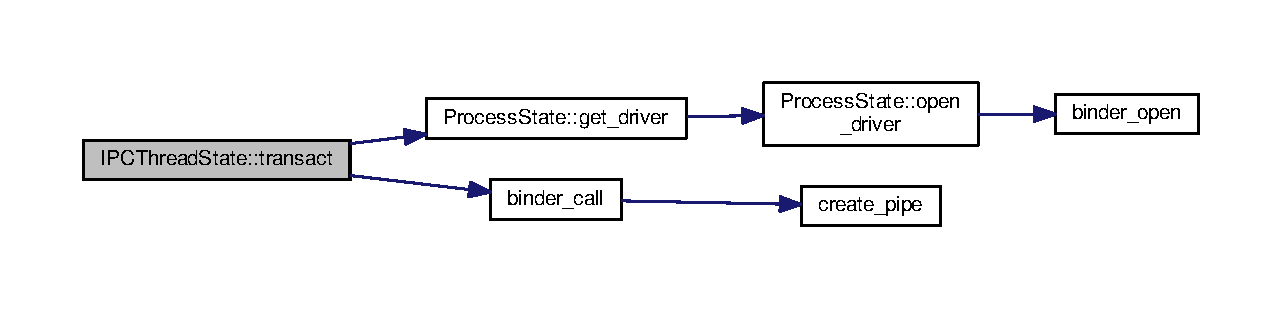
\includegraphics[width=350pt]{classIPCThreadState_a12423983ca5df01ecb79163ea3e0df82_cgraph}
\end{center}
\end{figure}




\subsection{Member Data Documentation}
\hypertarget{classIPCThreadState_a54fefc86880e0e140d40e9aa7247cc47}{\index{I\-P\-C\-Thread\-State@{I\-P\-C\-Thread\-State}!i\-Instance@{i\-Instance}}
\index{i\-Instance@{i\-Instance}!IPCThreadState@{I\-P\-C\-Thread\-State}}
\subsubsection[{i\-Instance}]{\setlength{\rightskip}{0pt plus 5cm}{\bf I\-P\-C\-Thread\-State} $\ast$ I\-P\-C\-Thread\-State\-::i\-Instance = 0\hspace{0.3cm}{\ttfamily [static]}, {\ttfamily [private]}}}\label{classIPCThreadState_a54fefc86880e0e140d40e9aa7247cc47}
\hypertarget{classIPCThreadState_aefae3c0f96244ce87f9289defee13b54}{\index{I\-P\-C\-Thread\-State@{I\-P\-C\-Thread\-State}!m\-Process@{m\-Process}}
\index{m\-Process@{m\-Process}!IPCThreadState@{I\-P\-C\-Thread\-State}}
\subsubsection[{m\-Process}]{\setlength{\rightskip}{0pt plus 5cm}{\bf Process\-State}$\ast$ I\-P\-C\-Thread\-State\-::m\-Process\hspace{0.3cm}{\ttfamily [private]}}}\label{classIPCThreadState_aefae3c0f96244ce87f9289defee13b54}


The documentation for this class was generated from the following file\-:\begin{DoxyCompactItemize}
\item 
\hyperlink{binder_8h}{binder.\-h}\end{DoxyCompactItemize}

\hypertarget{classProcessState}{\section{Process\-State Class Reference}
\label{classProcessState}\index{Process\-State@{Process\-State}}
}


{\ttfamily \#include $<$binder.\-h$>$}



Collaboration diagram for Process\-State\-:
\nopagebreak
\begin{figure}[H]
\begin{center}
\leavevmode
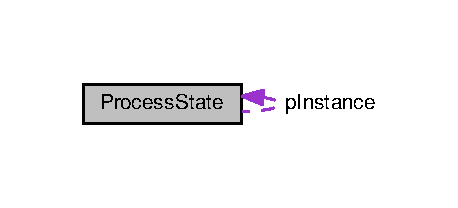
\includegraphics[width=220pt]{classProcessState__coll__graph}
\end{center}
\end{figure}
\subsection*{Public Member Functions}
\begin{DoxyCompactItemize}
\item 
int \hyperlink{classProcessState_ac89b9be4c5b62a0b4e0f9463b2cd5869}{get\-\_\-driver} ()
\item 
int \hyperlink{classProcessState_a466345e31d9732633daec40ae1143cef}{open\-\_\-driver} ()
\end{DoxyCompactItemize}
\subsection*{Static Public Member Functions}
\begin{DoxyCompactItemize}
\item 
static \hyperlink{classProcessState}{Process\-State} $\ast$ \hyperlink{classProcessState_a99f5eba7ab8777b26ebd837df67650f5}{self} ()
\end{DoxyCompactItemize}
\subsection*{Private Member Functions}
\begin{DoxyCompactItemize}
\item 
\hyperlink{classProcessState_a8359bb3ef4cb5c1ee1488757bf9d3b09}{Process\-State} ()
\item 
\hyperlink{classProcessState_a30cb15be9a906cf31816bd20ae452ab5}{Process\-State} (const \hyperlink{classProcessState}{Process\-State} \&p)
\item 
\hyperlink{classProcessState}{Process\-State} \& \hyperlink{classProcessState_a4ec70d27d0d7d45781809f71589ed1a5}{operator=} (const \hyperlink{classProcessState}{Process\-State} \&p)
\end{DoxyCompactItemize}
\subsection*{Private Attributes}
\begin{DoxyCompactItemize}
\item 
int \hyperlink{classProcessState_a76bd74bf501a4f428eee9555d1d3c493}{m\-Driver\-F\-D}
\end{DoxyCompactItemize}
\subsection*{Static Private Attributes}
\begin{DoxyCompactItemize}
\item 
static \hyperlink{classProcessState}{Process\-State} $\ast$ \hyperlink{classProcessState_a85d9fa40156e923969fcb00ffdc3ab1a}{p\-Instance} = 0
\end{DoxyCompactItemize}


\subsection{Constructor \& Destructor Documentation}
\hypertarget{classProcessState_a8359bb3ef4cb5c1ee1488757bf9d3b09}{\index{Process\-State@{Process\-State}!Process\-State@{Process\-State}}
\index{Process\-State@{Process\-State}!ProcessState@{Process\-State}}
\subsubsection[{Process\-State}]{\setlength{\rightskip}{0pt plus 5cm}Process\-State\-::\-Process\-State (
\begin{DoxyParamCaption}
{}
\end{DoxyParamCaption}
)\hspace{0.3cm}{\ttfamily [inline]}, {\ttfamily [private]}}}\label{classProcessState_a8359bb3ef4cb5c1ee1488757bf9d3b09}
\hypertarget{classProcessState_a30cb15be9a906cf31816bd20ae452ab5}{\index{Process\-State@{Process\-State}!Process\-State@{Process\-State}}
\index{Process\-State@{Process\-State}!ProcessState@{Process\-State}}
\subsubsection[{Process\-State}]{\setlength{\rightskip}{0pt plus 5cm}Process\-State\-::\-Process\-State (
\begin{DoxyParamCaption}
\item[{const {\bf Process\-State} \&}]{p}
\end{DoxyParamCaption}
)\hspace{0.3cm}{\ttfamily [private]}}}\label{classProcessState_a30cb15be9a906cf31816bd20ae452ab5}


\subsection{Member Function Documentation}
\hypertarget{classProcessState_ac89b9be4c5b62a0b4e0f9463b2cd5869}{\index{Process\-State@{Process\-State}!get\-\_\-driver@{get\-\_\-driver}}
\index{get\-\_\-driver@{get\-\_\-driver}!ProcessState@{Process\-State}}
\subsubsection[{get\-\_\-driver}]{\setlength{\rightskip}{0pt plus 5cm}int Process\-State\-::get\-\_\-driver (
\begin{DoxyParamCaption}
{}
\end{DoxyParamCaption}
)\hspace{0.3cm}{\ttfamily [inline]}}}\label{classProcessState_ac89b9be4c5b62a0b4e0f9463b2cd5869}


Here is the call graph for this function\-:
\nopagebreak
\begin{figure}[H]
\begin{center}
\leavevmode
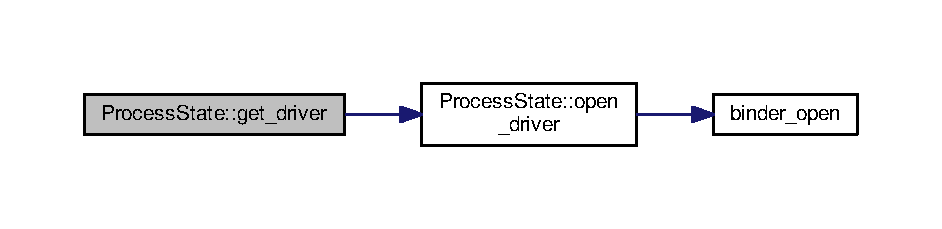
\includegraphics[width=350pt]{classProcessState_ac89b9be4c5b62a0b4e0f9463b2cd5869_cgraph}
\end{center}
\end{figure}


\hypertarget{classProcessState_a466345e31d9732633daec40ae1143cef}{\index{Process\-State@{Process\-State}!open\-\_\-driver@{open\-\_\-driver}}
\index{open\-\_\-driver@{open\-\_\-driver}!ProcessState@{Process\-State}}
\subsubsection[{open\-\_\-driver}]{\setlength{\rightskip}{0pt plus 5cm}int Process\-State\-::open\-\_\-driver (
\begin{DoxyParamCaption}
{}
\end{DoxyParamCaption}
)\hspace{0.3cm}{\ttfamily [inline]}}}\label{classProcessState_a466345e31d9732633daec40ae1143cef}


Here is the call graph for this function\-:
\nopagebreak
\begin{figure}[H]
\begin{center}
\leavevmode
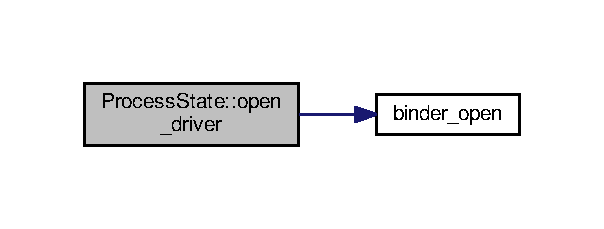
\includegraphics[width=290pt]{classProcessState_a466345e31d9732633daec40ae1143cef_cgraph}
\end{center}
\end{figure}


\hypertarget{classProcessState_a4ec70d27d0d7d45781809f71589ed1a5}{\index{Process\-State@{Process\-State}!operator=@{operator=}}
\index{operator=@{operator=}!ProcessState@{Process\-State}}
\subsubsection[{operator=}]{\setlength{\rightskip}{0pt plus 5cm}{\bf Process\-State}\& Process\-State\-::operator= (
\begin{DoxyParamCaption}
\item[{const {\bf Process\-State} \&}]{p}
\end{DoxyParamCaption}
)\hspace{0.3cm}{\ttfamily [private]}}}\label{classProcessState_a4ec70d27d0d7d45781809f71589ed1a5}
\hypertarget{classProcessState_a99f5eba7ab8777b26ebd837df67650f5}{\index{Process\-State@{Process\-State}!self@{self}}
\index{self@{self}!ProcessState@{Process\-State}}
\subsubsection[{self}]{\setlength{\rightskip}{0pt plus 5cm}static {\bf Process\-State}$\ast$ Process\-State\-::self (
\begin{DoxyParamCaption}
{}
\end{DoxyParamCaption}
)\hspace{0.3cm}{\ttfamily [inline]}, {\ttfamily [static]}}}\label{classProcessState_a99f5eba7ab8777b26ebd837df67650f5}


Here is the call graph for this function\-:
\nopagebreak
\begin{figure}[H]
\begin{center}
\leavevmode
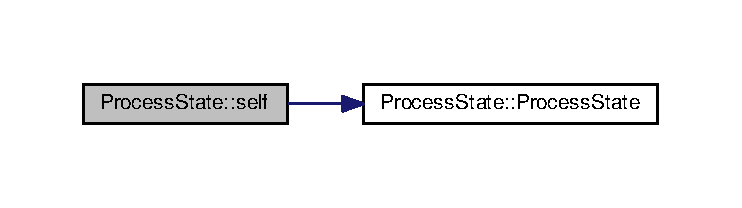
\includegraphics[width=350pt]{classProcessState_a99f5eba7ab8777b26ebd837df67650f5_cgraph}
\end{center}
\end{figure}




\subsection{Member Data Documentation}
\hypertarget{classProcessState_a76bd74bf501a4f428eee9555d1d3c493}{\index{Process\-State@{Process\-State}!m\-Driver\-F\-D@{m\-Driver\-F\-D}}
\index{m\-Driver\-F\-D@{m\-Driver\-F\-D}!ProcessState@{Process\-State}}
\subsubsection[{m\-Driver\-F\-D}]{\setlength{\rightskip}{0pt plus 5cm}int Process\-State\-::m\-Driver\-F\-D\hspace{0.3cm}{\ttfamily [private]}}}\label{classProcessState_a76bd74bf501a4f428eee9555d1d3c493}
\hypertarget{classProcessState_a85d9fa40156e923969fcb00ffdc3ab1a}{\index{Process\-State@{Process\-State}!p\-Instance@{p\-Instance}}
\index{p\-Instance@{p\-Instance}!ProcessState@{Process\-State}}
\subsubsection[{p\-Instance}]{\setlength{\rightskip}{0pt plus 5cm}{\bf Process\-State} $\ast$ Process\-State\-::p\-Instance = 0\hspace{0.3cm}{\ttfamily [static]}, {\ttfamily [private]}}}\label{classProcessState_a85d9fa40156e923969fcb00ffdc3ab1a}


The documentation for this class was generated from the following file\-:\begin{DoxyCompactItemize}
\item 
\hyperlink{binder_8h}{binder.\-h}\end{DoxyCompactItemize}

\chapter{File Documentation}
\hypertarget{binder_8h}{\section{binder.\-h File Reference}
\label{binder_8h}\index{binder.\-h@{binder.\-h}}
}
{\ttfamily \#include $<$sys/types.\-h$>$}\\*
{\ttfamily \#include $<$sys/stat.\-h$>$}\\*
{\ttfamily \#include $<$fcntl.\-h$>$}\\*
{\ttfamily \#include $<$unistd.\-h$>$}\\*
{\ttfamily \#include $<$stdio.\-h$>$}\\*
{\ttfamily \#include $<$stdlib.\-h$>$}\\*
{\ttfamily \#include $<$errno.\-h$>$}\\*
Include dependency graph for binder.\-h\-:
\nopagebreak
\begin{figure}[H]
\begin{center}
\leavevmode
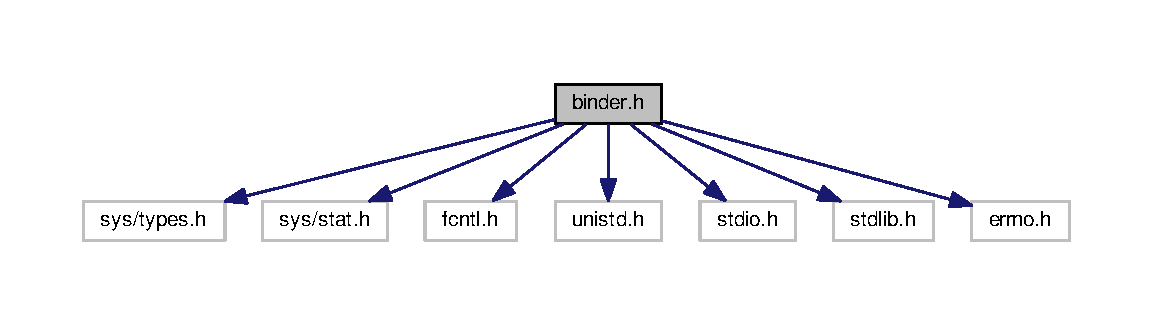
\includegraphics[width=350pt]{binder_8h__incl}
\end{center}
\end{figure}
\subsection*{Classes}
\begin{DoxyCompactItemize}
\item 
class \hyperlink{classProcessState}{Process\-State}
\item 
class \hyperlink{classIBinder}{I\-Binder}
\item 
class \hyperlink{classBBinder}{B\-Binder}
\item 
class \hyperlink{classBnInterface}{Bn\-Interface$<$ I\-N\-T\-E\-R\-F\-A\-C\-E $>$}
\item 
class \hyperlink{classIPCThreadState}{I\-P\-C\-Thread\-State}
\item 
class \hyperlink{classBpBinder}{Bp\-Binder}
\item 
class \hyperlink{classBpRefBase}{Bp\-Ref\-Base}
\item 
class \hyperlink{classIInterface}{I\-Interface}
\item 
class \hyperlink{classILedService}{I\-Led\-Service}
\item 
class \hyperlink{classBpInterface}{Bp\-Interface$<$ I\-N\-T\-E\-R\-F\-A\-C\-E $>$}
\end{DoxyCompactItemize}
\subsection*{Macros}
\begin{DoxyCompactItemize}
\item 
\#define \hyperlink{binder_8h_affb243347b149536c185539e260a4e5b}{B\-I\-N\-D\-E\-R\-\_\-\-S\-E\-R\-V\-I\-C\-E\-\_\-\-M\-A\-N\-A\-G\-E\-R}~0
\item 
\#define \hyperlink{binder_8h_a94901f8e52275fe27b50b94f8b2602cb}{S\-V\-C\-\_\-\-M\-G\-R\-\_\-\-A\-D\-D\-\_\-\-S\-E\-R\-V\-I\-C\-E}~0x\-F\-F\-F\-F\-F\-F\-F0
\item 
\#define \hyperlink{binder_8h_ac86e2cbabb68dfb96c6de13be54c09de}{S\-V\-C\-\_\-\-M\-G\-R\-\_\-\-C\-H\-E\-C\-K\-\_\-\-S\-E\-R\-V\-I\-C\-E}~0x\-F\-F\-F\-F\-F\-F\-F1
\item 
\#define \hyperlink{binder_8h_aa04c9b86c0af7318cda857aa84cc28b8}{B\-I\-N\-D\-E\-R\-\_\-\-P\-A\-T\-H}~\char`\"{}/tmp/binder\char`\"{}
\item 
\#define \hyperlink{binder_8h_af5ab3506a20d58ad1faf58a481207869}{D\-E\-C\-L\-A\-R\-E\-\_\-\-M\-E\-T\-A\-\_\-\-I\-N\-T\-E\-R\-F\-A\-C\-E}(I\-N\-T\-E\-R\-F\-A\-C\-E)~static I\#\#I\-N\-T\-E\-R\-F\-A\-C\-E $\ast$as\-Interface(\hyperlink{classIBinder}{I\-Binder} $\ast$p)
\item 
\#define \hyperlink{binder_8h_ac30579507560c91b8b5249230f6bab4b}{I\-M\-P\-L\-E\-M\-E\-N\-T\-\_\-\-M\-E\-T\-A\-\_\-\-I\-N\-T\-E\-R\-F\-A\-C\-E}(I\-N\-T\-E\-R\-F\-A\-C\-E)~I\#\#I\-N\-T\-E\-R\-F\-A\-C\-E $\ast$I\#\#I\-N\-T\-E\-R\-F\-A\-C\-E\-::as\-Interface(\hyperlink{classIBinder}{I\-Binder} $\ast$p) \{ return new Bp\#\#I\-N\-T\-E\-R\-F\-A\-C\-E(p); \}
\end{DoxyCompactItemize}
\subsection*{Typedefs}
\begin{DoxyCompactItemize}
\item 
typedef int($\ast$ \hyperlink{binder_8h_a1746f77853bbabef2a622bc86f53a4ad}{binder\-\_\-handler} )(int code, int msg, int $\ast$reply)
\end{DoxyCompactItemize}
\subsection*{Functions}
\begin{DoxyCompactItemize}
\item 
int \hyperlink{binder_8h_aa95623d68fe666d523c2f7b31ff6e775}{binder\-\_\-open} (int mapsize)
\item 
int \hyperlink{binder_8h_a353da2e2685b66ecd6e4457c1ff3ae45}{create\-\_\-pipe} (const char $\ast$path, int mode)
\item 
int \hyperlink{binder_8h_a100a49cf142a7bbc7a93fe120ae2e973}{binder\-\_\-call} (int binder, int $\ast$msg, int $\ast$reply, int target, int code)
\item 
void \hyperlink{binder_8h_a3f3d2bf50652a6baa7de13ac4aceb7a5}{binder\-\_\-loop} (int binder, \hyperlink{binder_8h_a1746f77853bbabef2a622bc86f53a4ad}{binder\-\_\-handler} func)
\item 
void \hyperlink{binder_8h_af566fd57f21343a030ff8876cfa65950}{add\-Service} (const char $\ast$name, \hyperlink{classIBinder}{I\-Binder} $\ast$p)
\item 
\hyperlink{classIBinder}{I\-Binder} $\ast$ \hyperlink{binder_8h_a51fbbc00e7e7bd7953d3267af704a868}{get\-Service} (const char $\ast$name)
\item 
{\footnotesize template$<$typename I\-N\-T\-E\-R\-F\-A\-C\-E $>$ }\\I\-N\-T\-E\-R\-F\-A\-C\-E $\ast$ \hyperlink{binder_8h_a90e858387208e85b605a427d03a77e4d}{interface\-\_\-cast} (\hyperlink{classIBinder}{I\-Binder} $\ast$p)
\end{DoxyCompactItemize}
\subsection*{Variables}
\begin{DoxyCompactItemize}
\item 
bool \hyperlink{binder_8h_ae948c0e495cb4246e8f4de881699c194}{server\-\_\-init} = false
\item 
bool \hyperlink{binder_8h_aa0df924d0a93af9346ecfa560b7ed264}{client\-\_\-init} = false
\item 
int \hyperlink{binder_8h_a975a11a8517c6a028111ed3694100ac0}{binder\-\_\-fd} = 0
\item 
const char $\ast$ \hyperlink{binder_8h_ade69e82a5c88f18b279db12ba553d83f}{service\-\_\-name}
\item 
\hyperlink{classIBinder}{I\-Binder} $\ast$ \hyperlink{binder_8h_a43a7671f7a99c62d39930b130991a3e9}{server}
\end{DoxyCompactItemize}


\subsection{Macro Definition Documentation}
\hypertarget{binder_8h_aa04c9b86c0af7318cda857aa84cc28b8}{\index{binder.\-h@{binder.\-h}!B\-I\-N\-D\-E\-R\-\_\-\-P\-A\-T\-H@{B\-I\-N\-D\-E\-R\-\_\-\-P\-A\-T\-H}}
\index{B\-I\-N\-D\-E\-R\-\_\-\-P\-A\-T\-H@{B\-I\-N\-D\-E\-R\-\_\-\-P\-A\-T\-H}!binder.h@{binder.\-h}}
\subsubsection[{B\-I\-N\-D\-E\-R\-\_\-\-P\-A\-T\-H}]{\setlength{\rightskip}{0pt plus 5cm}\#define B\-I\-N\-D\-E\-R\-\_\-\-P\-A\-T\-H~\char`\"{}/tmp/binder\char`\"{}}}\label{binder_8h_aa04c9b86c0af7318cda857aa84cc28b8}
\hypertarget{binder_8h_affb243347b149536c185539e260a4e5b}{\index{binder.\-h@{binder.\-h}!B\-I\-N\-D\-E\-R\-\_\-\-S\-E\-R\-V\-I\-C\-E\-\_\-\-M\-A\-N\-A\-G\-E\-R@{B\-I\-N\-D\-E\-R\-\_\-\-S\-E\-R\-V\-I\-C\-E\-\_\-\-M\-A\-N\-A\-G\-E\-R}}
\index{B\-I\-N\-D\-E\-R\-\_\-\-S\-E\-R\-V\-I\-C\-E\-\_\-\-M\-A\-N\-A\-G\-E\-R@{B\-I\-N\-D\-E\-R\-\_\-\-S\-E\-R\-V\-I\-C\-E\-\_\-\-M\-A\-N\-A\-G\-E\-R}!binder.h@{binder.\-h}}
\subsubsection[{B\-I\-N\-D\-E\-R\-\_\-\-S\-E\-R\-V\-I\-C\-E\-\_\-\-M\-A\-N\-A\-G\-E\-R}]{\setlength{\rightskip}{0pt plus 5cm}\#define B\-I\-N\-D\-E\-R\-\_\-\-S\-E\-R\-V\-I\-C\-E\-\_\-\-M\-A\-N\-A\-G\-E\-R~0}}\label{binder_8h_affb243347b149536c185539e260a4e5b}
\hypertarget{binder_8h_af5ab3506a20d58ad1faf58a481207869}{\index{binder.\-h@{binder.\-h}!D\-E\-C\-L\-A\-R\-E\-\_\-\-M\-E\-T\-A\-\_\-\-I\-N\-T\-E\-R\-F\-A\-C\-E@{D\-E\-C\-L\-A\-R\-E\-\_\-\-M\-E\-T\-A\-\_\-\-I\-N\-T\-E\-R\-F\-A\-C\-E}}
\index{D\-E\-C\-L\-A\-R\-E\-\_\-\-M\-E\-T\-A\-\_\-\-I\-N\-T\-E\-R\-F\-A\-C\-E@{D\-E\-C\-L\-A\-R\-E\-\_\-\-M\-E\-T\-A\-\_\-\-I\-N\-T\-E\-R\-F\-A\-C\-E}!binder.h@{binder.\-h}}
\subsubsection[{D\-E\-C\-L\-A\-R\-E\-\_\-\-M\-E\-T\-A\-\_\-\-I\-N\-T\-E\-R\-F\-A\-C\-E}]{\setlength{\rightskip}{0pt plus 5cm}\#define D\-E\-C\-L\-A\-R\-E\-\_\-\-M\-E\-T\-A\-\_\-\-I\-N\-T\-E\-R\-F\-A\-C\-E(
\begin{DoxyParamCaption}
\item[{}]{I\-N\-T\-E\-R\-F\-A\-C\-E}
\end{DoxyParamCaption}
)~static I\#\#I\-N\-T\-E\-R\-F\-A\-C\-E $\ast$as\-Interface({\bf I\-Binder} $\ast$p)}}\label{binder_8h_af5ab3506a20d58ad1faf58a481207869}
\hypertarget{binder_8h_ac30579507560c91b8b5249230f6bab4b}{\index{binder.\-h@{binder.\-h}!I\-M\-P\-L\-E\-M\-E\-N\-T\-\_\-\-M\-E\-T\-A\-\_\-\-I\-N\-T\-E\-R\-F\-A\-C\-E@{I\-M\-P\-L\-E\-M\-E\-N\-T\-\_\-\-M\-E\-T\-A\-\_\-\-I\-N\-T\-E\-R\-F\-A\-C\-E}}
\index{I\-M\-P\-L\-E\-M\-E\-N\-T\-\_\-\-M\-E\-T\-A\-\_\-\-I\-N\-T\-E\-R\-F\-A\-C\-E@{I\-M\-P\-L\-E\-M\-E\-N\-T\-\_\-\-M\-E\-T\-A\-\_\-\-I\-N\-T\-E\-R\-F\-A\-C\-E}!binder.h@{binder.\-h}}
\subsubsection[{I\-M\-P\-L\-E\-M\-E\-N\-T\-\_\-\-M\-E\-T\-A\-\_\-\-I\-N\-T\-E\-R\-F\-A\-C\-E}]{\setlength{\rightskip}{0pt plus 5cm}\#define I\-M\-P\-L\-E\-M\-E\-N\-T\-\_\-\-M\-E\-T\-A\-\_\-\-I\-N\-T\-E\-R\-F\-A\-C\-E(
\begin{DoxyParamCaption}
\item[{}]{I\-N\-T\-E\-R\-F\-A\-C\-E}
\end{DoxyParamCaption}
)~I\#\#I\-N\-T\-E\-R\-F\-A\-C\-E $\ast$I\#\#I\-N\-T\-E\-R\-F\-A\-C\-E\-::as\-Interface({\bf I\-Binder} $\ast$p) \{ return new Bp\#\#I\-N\-T\-E\-R\-F\-A\-C\-E(p); \}}}\label{binder_8h_ac30579507560c91b8b5249230f6bab4b}
\hypertarget{binder_8h_a94901f8e52275fe27b50b94f8b2602cb}{\index{binder.\-h@{binder.\-h}!S\-V\-C\-\_\-\-M\-G\-R\-\_\-\-A\-D\-D\-\_\-\-S\-E\-R\-V\-I\-C\-E@{S\-V\-C\-\_\-\-M\-G\-R\-\_\-\-A\-D\-D\-\_\-\-S\-E\-R\-V\-I\-C\-E}}
\index{S\-V\-C\-\_\-\-M\-G\-R\-\_\-\-A\-D\-D\-\_\-\-S\-E\-R\-V\-I\-C\-E@{S\-V\-C\-\_\-\-M\-G\-R\-\_\-\-A\-D\-D\-\_\-\-S\-E\-R\-V\-I\-C\-E}!binder.h@{binder.\-h}}
\subsubsection[{S\-V\-C\-\_\-\-M\-G\-R\-\_\-\-A\-D\-D\-\_\-\-S\-E\-R\-V\-I\-C\-E}]{\setlength{\rightskip}{0pt plus 5cm}\#define S\-V\-C\-\_\-\-M\-G\-R\-\_\-\-A\-D\-D\-\_\-\-S\-E\-R\-V\-I\-C\-E~0x\-F\-F\-F\-F\-F\-F\-F0}}\label{binder_8h_a94901f8e52275fe27b50b94f8b2602cb}
\hypertarget{binder_8h_ac86e2cbabb68dfb96c6de13be54c09de}{\index{binder.\-h@{binder.\-h}!S\-V\-C\-\_\-\-M\-G\-R\-\_\-\-C\-H\-E\-C\-K\-\_\-\-S\-E\-R\-V\-I\-C\-E@{S\-V\-C\-\_\-\-M\-G\-R\-\_\-\-C\-H\-E\-C\-K\-\_\-\-S\-E\-R\-V\-I\-C\-E}}
\index{S\-V\-C\-\_\-\-M\-G\-R\-\_\-\-C\-H\-E\-C\-K\-\_\-\-S\-E\-R\-V\-I\-C\-E@{S\-V\-C\-\_\-\-M\-G\-R\-\_\-\-C\-H\-E\-C\-K\-\_\-\-S\-E\-R\-V\-I\-C\-E}!binder.h@{binder.\-h}}
\subsubsection[{S\-V\-C\-\_\-\-M\-G\-R\-\_\-\-C\-H\-E\-C\-K\-\_\-\-S\-E\-R\-V\-I\-C\-E}]{\setlength{\rightskip}{0pt plus 5cm}\#define S\-V\-C\-\_\-\-M\-G\-R\-\_\-\-C\-H\-E\-C\-K\-\_\-\-S\-E\-R\-V\-I\-C\-E~0x\-F\-F\-F\-F\-F\-F\-F1}}\label{binder_8h_ac86e2cbabb68dfb96c6de13be54c09de}


\subsection{Typedef Documentation}
\hypertarget{binder_8h_a1746f77853bbabef2a622bc86f53a4ad}{\index{binder.\-h@{binder.\-h}!binder\-\_\-handler@{binder\-\_\-handler}}
\index{binder\-\_\-handler@{binder\-\_\-handler}!binder.h@{binder.\-h}}
\subsubsection[{binder\-\_\-handler}]{\setlength{\rightskip}{0pt plus 5cm}typedef int($\ast$ binder\-\_\-handler)(int code, int msg, int $\ast$reply)}}\label{binder_8h_a1746f77853bbabef2a622bc86f53a4ad}


\subsection{Function Documentation}
\hypertarget{binder_8h_af566fd57f21343a030ff8876cfa65950}{\index{binder.\-h@{binder.\-h}!add\-Service@{add\-Service}}
\index{add\-Service@{add\-Service}!binder.h@{binder.\-h}}
\subsubsection[{add\-Service}]{\setlength{\rightskip}{0pt plus 5cm}void add\-Service (
\begin{DoxyParamCaption}
\item[{const char $\ast$}]{name, }
\item[{{\bf I\-Binder} $\ast$}]{p}
\end{DoxyParamCaption}
)}}\label{binder_8h_af566fd57f21343a030ff8876cfa65950}


Here is the call graph for this function\-:
\nopagebreak
\begin{figure}[H]
\begin{center}
\leavevmode
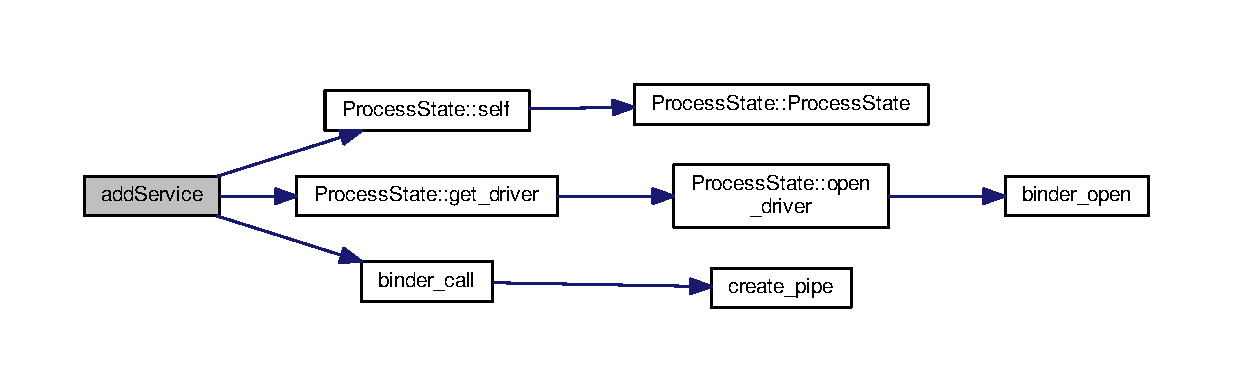
\includegraphics[width=350pt]{binder_8h_af566fd57f21343a030ff8876cfa65950_cgraph}
\end{center}
\end{figure}


\hypertarget{binder_8h_a100a49cf142a7bbc7a93fe120ae2e973}{\index{binder.\-h@{binder.\-h}!binder\-\_\-call@{binder\-\_\-call}}
\index{binder\-\_\-call@{binder\-\_\-call}!binder.h@{binder.\-h}}
\subsubsection[{binder\-\_\-call}]{\setlength{\rightskip}{0pt plus 5cm}int binder\-\_\-call (
\begin{DoxyParamCaption}
\item[{int}]{binder, }
\item[{int $\ast$}]{msg, }
\item[{int $\ast$}]{reply, }
\item[{int}]{target, }
\item[{int}]{code}
\end{DoxyParamCaption}
)}}\label{binder_8h_a100a49cf142a7bbc7a93fe120ae2e973}


Here is the call graph for this function\-:
\nopagebreak
\begin{figure}[H]
\begin{center}
\leavevmode
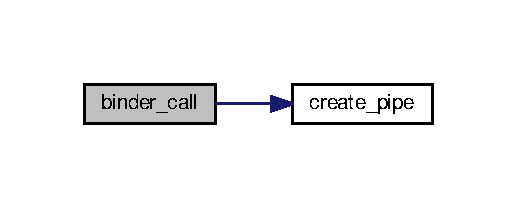
\includegraphics[width=248pt]{binder_8h_a100a49cf142a7bbc7a93fe120ae2e973_cgraph}
\end{center}
\end{figure}


\hypertarget{binder_8h_a3f3d2bf50652a6baa7de13ac4aceb7a5}{\index{binder.\-h@{binder.\-h}!binder\-\_\-loop@{binder\-\_\-loop}}
\index{binder\-\_\-loop@{binder\-\_\-loop}!binder.h@{binder.\-h}}
\subsubsection[{binder\-\_\-loop}]{\setlength{\rightskip}{0pt plus 5cm}void binder\-\_\-loop (
\begin{DoxyParamCaption}
\item[{int}]{binder, }
\item[{{\bf binder\-\_\-handler}}]{func}
\end{DoxyParamCaption}
)}}\label{binder_8h_a3f3d2bf50652a6baa7de13ac4aceb7a5}
\hypertarget{binder_8h_aa95623d68fe666d523c2f7b31ff6e775}{\index{binder.\-h@{binder.\-h}!binder\-\_\-open@{binder\-\_\-open}}
\index{binder\-\_\-open@{binder\-\_\-open}!binder.h@{binder.\-h}}
\subsubsection[{binder\-\_\-open}]{\setlength{\rightskip}{0pt plus 5cm}int binder\-\_\-open (
\begin{DoxyParamCaption}
\item[{int}]{mapsize}
\end{DoxyParamCaption}
)}}\label{binder_8h_aa95623d68fe666d523c2f7b31ff6e775}
\hypertarget{binder_8h_a353da2e2685b66ecd6e4457c1ff3ae45}{\index{binder.\-h@{binder.\-h}!create\-\_\-pipe@{create\-\_\-pipe}}
\index{create\-\_\-pipe@{create\-\_\-pipe}!binder.h@{binder.\-h}}
\subsubsection[{create\-\_\-pipe}]{\setlength{\rightskip}{0pt plus 5cm}int create\-\_\-pipe (
\begin{DoxyParamCaption}
\item[{const char $\ast$}]{path, }
\item[{int}]{mode}
\end{DoxyParamCaption}
)}}\label{binder_8h_a353da2e2685b66ecd6e4457c1ff3ae45}
\hypertarget{binder_8h_a51fbbc00e7e7bd7953d3267af704a868}{\index{binder.\-h@{binder.\-h}!get\-Service@{get\-Service}}
\index{get\-Service@{get\-Service}!binder.h@{binder.\-h}}
\subsubsection[{get\-Service}]{\setlength{\rightskip}{0pt plus 5cm}{\bf I\-Binder}$\ast$ get\-Service (
\begin{DoxyParamCaption}
\item[{const char $\ast$}]{name}
\end{DoxyParamCaption}
)}}\label{binder_8h_a51fbbc00e7e7bd7953d3267af704a868}


Here is the call graph for this function\-:
\nopagebreak
\begin{figure}[H]
\begin{center}
\leavevmode
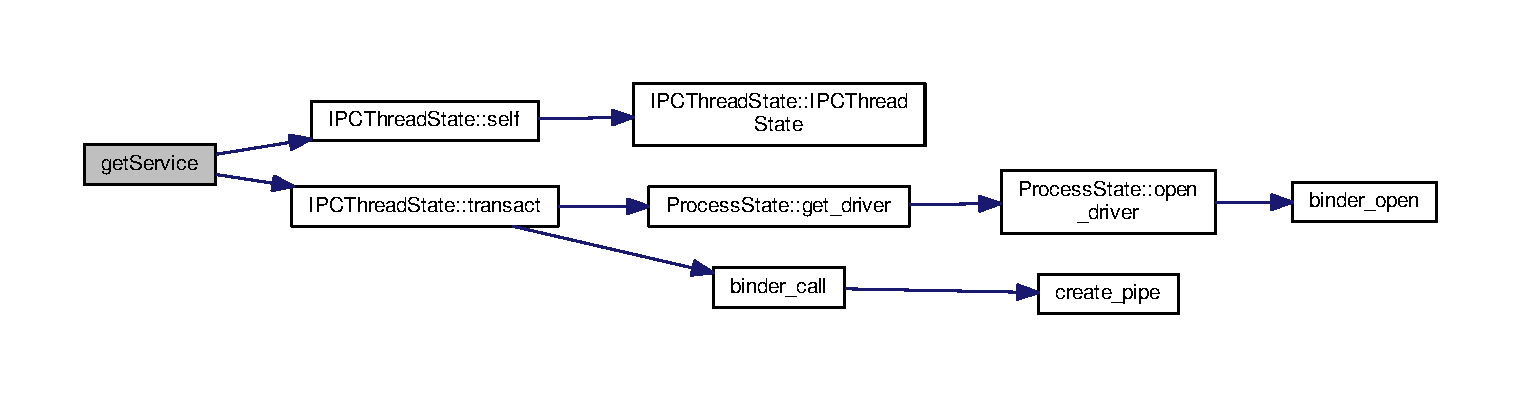
\includegraphics[width=350pt]{binder_8h_a51fbbc00e7e7bd7953d3267af704a868_cgraph}
\end{center}
\end{figure}


\hypertarget{binder_8h_a90e858387208e85b605a427d03a77e4d}{\index{binder.\-h@{binder.\-h}!interface\-\_\-cast@{interface\-\_\-cast}}
\index{interface\-\_\-cast@{interface\-\_\-cast}!binder.h@{binder.\-h}}
\subsubsection[{interface\-\_\-cast}]{\setlength{\rightskip}{0pt plus 5cm}template$<$typename I\-N\-T\-E\-R\-F\-A\-C\-E $>$ I\-N\-T\-E\-R\-F\-A\-C\-E$\ast$ interface\-\_\-cast (
\begin{DoxyParamCaption}
\item[{{\bf I\-Binder} $\ast$}]{p}
\end{DoxyParamCaption}
)}}\label{binder_8h_a90e858387208e85b605a427d03a77e4d}


\subsection{Variable Documentation}
\hypertarget{binder_8h_a975a11a8517c6a028111ed3694100ac0}{\index{binder.\-h@{binder.\-h}!binder\-\_\-fd@{binder\-\_\-fd}}
\index{binder\-\_\-fd@{binder\-\_\-fd}!binder.h@{binder.\-h}}
\subsubsection[{binder\-\_\-fd}]{\setlength{\rightskip}{0pt plus 5cm}int binder\-\_\-fd = 0}}\label{binder_8h_a975a11a8517c6a028111ed3694100ac0}
\hypertarget{binder_8h_aa0df924d0a93af9346ecfa560b7ed264}{\index{binder.\-h@{binder.\-h}!client\-\_\-init@{client\-\_\-init}}
\index{client\-\_\-init@{client\-\_\-init}!binder.h@{binder.\-h}}
\subsubsection[{client\-\_\-init}]{\setlength{\rightskip}{0pt plus 5cm}bool client\-\_\-init = false}}\label{binder_8h_aa0df924d0a93af9346ecfa560b7ed264}
\hypertarget{binder_8h_a43a7671f7a99c62d39930b130991a3e9}{\index{binder.\-h@{binder.\-h}!server@{server}}
\index{server@{server}!binder.h@{binder.\-h}}
\subsubsection[{server}]{\setlength{\rightskip}{0pt plus 5cm}{\bf I\-Binder}$\ast$ server}}\label{binder_8h_a43a7671f7a99c62d39930b130991a3e9}
\hypertarget{binder_8h_ae948c0e495cb4246e8f4de881699c194}{\index{binder.\-h@{binder.\-h}!server\-\_\-init@{server\-\_\-init}}
\index{server\-\_\-init@{server\-\_\-init}!binder.h@{binder.\-h}}
\subsubsection[{server\-\_\-init}]{\setlength{\rightskip}{0pt plus 5cm}bool server\-\_\-init = false}}\label{binder_8h_ae948c0e495cb4246e8f4de881699c194}
\hypertarget{binder_8h_ade69e82a5c88f18b279db12ba553d83f}{\index{binder.\-h@{binder.\-h}!service\-\_\-name@{service\-\_\-name}}
\index{service\-\_\-name@{service\-\_\-name}!binder.h@{binder.\-h}}
\subsubsection[{service\-\_\-name}]{\setlength{\rightskip}{0pt plus 5cm}const char$\ast$ service\-\_\-name}}\label{binder_8h_ade69e82a5c88f18b279db12ba553d83f}

%--- End generated contents ---

% Index
\newpage
\phantomsection
\addcontentsline{toc}{chapter}{Index}
\printindex

\end{document}
